%!TEX root = ../sztuthesis_main.tex
% 论文正文是主体,主体部分应从另页右页开始,每一章应另起页。一般由序号标题、文字叙述、图、表格和公式等五个部分构成。
\section{引言}
\subsection{研究背景与意义}

心血管疾病(CVD),包括心脏病、高血压、心律失常等症状,已成为居民自然死亡原因中的一部分。根据《中国心血管健康与疾病报告2022概要》 \cite{中国心血管健康与疾病报告2022概要} 的数据,我国CVD的发病率以及死亡率逐年提高,按所引用的报告推算,截止2022年,我国CVD患者现患人数有3.3亿之多,我国城镇和乡村居民人口因心血管疾病造成的死亡人数约占城乡居民疾病死亡构成比的二分之一。在此背景下,早期发现、诊断和及时治疗心脏病变,尤其是通过长期的心电监测手段去提前预警心脏病变情况,已成为预防心血管疾病,拯救患者生命的关键。

心脏的器官壁主要是由心肌构成的。这种肌肉的特征表现和人体关节以及四肢上的骨骼肌肉是一样的,但和血管、肠胃等器官里那些由平滑肌构成的器官不同。心脏具有将血液泵向全身的作用,将血液中的氧气输送到全身各组织中。而控制这种泵动作用的神经信号是心肌电,心肌电产生的活动电位扩散到整个心脏,心肌受到刺激后发生收缩,进而导致心脏的机械活动,即心跳。在每一个心跳周期中,心肌电电信号变化的方向,大小和时间都有规律可循,这种规律的变化,可以通过心电图来反映出来。心电图是通过记录心肌电变化所产生的活动电位在体内流动,使用心电图机(electrocardiograph)用适当的方法(如导联)将其记录下来的图形,叫做心电图(electrocardiogram,ECG)。如图\ref{F.ECG_image}所示。心电图是临床上诊断心脏疾病的重要手段之一,通过心电图可以了解心脏的生理和病理状态,对心脏疾病的诊断、鉴别诊断、疗效评价和预后判断有重要的临床意义。心电图是一种无创性检查方法,操作简便,费用低廉,且无辐射,对患者无损害,因此在临床上得到广泛应用。

\begin{figure}[hbt]
    \centering
    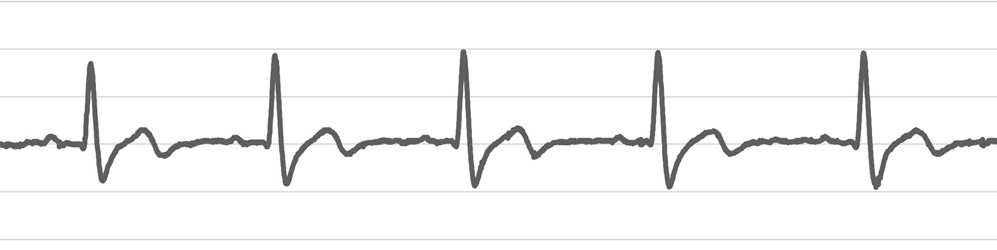
\includegraphics[width=0.7\textwidth]{image1.jpg}
    \caption{心电图示例}
    \label{F.ECG_image}
\end{figure}

然而,通过使用固定式心电图机来进行心电图检测的现状仍面临一些局限,尤其是在便捷性和实时性方面。此种心电图检测设备通常需要患者到医院进行检查,这种方式不仅会占用患者大量的时间,还容易造成患者的心电数据在长时间内的缺失或延迟获取。

许多心血管问题,尤其是窦性心动过速、期前早搏、心房颤动等症状,往往是间歇性或不规律发生的。传统的心电图检测只能进行点对点测量,即患者在特定的时间和地点进行一次性检测,这样无法捕捉到心脏在不同时间段的动态变化,如患者在进食、工作、运动等状态下的心电信息。对于一些潜在的心脏问题,医生往往无法通过单次检查做出全面准确的判断。

如在心血管研究中 \cite{高强度负荷训练对新入伍战士动态心电图相关指标的影响} ,对大量样本的实时同步心电采集的需求逐渐突出,由于传统设备只能同时采集个数样本,所采样本数据难以兼顾时基一致性问题。通过发展无线心电同步采集技术,能够通过无线网络将多台设备同步连接,实时采集患者的心电数据,解决了传统设备空间和连接限制的问题。尤其在大规模监测、远程医疗、运动医学以及急救等领域,无线多心电同步采集设备具有广阔的应用前景 \cite{物联网技术在智能医疗监护与康复辅助设备中的应用探索}。

在国外对无线心电测量的研究中,随着无线射频通信技术和心电监测设备的不断进步,无线多心电同步采集系统已经成为心电监护领域的一大研究方向。早期的心电监测设备大多笨重且运行功耗较大,需要使用大量导联线连接,存在安装和使用不便等缺点。而现代无线心电监测设备通过WiFi \cite{基于Wi-Fi的医疗设备物联网采集装置设计} 、蓝牙 \cite{KhoBesar-34} 、Zigbee \cite{I.H.-35} 等无线协议,实现了设备之间的无线互联和远程监控。

国内无线心电同步采集设备的研究较少,早期研究多为针对简化数据采集方式的研究,如基于有线通信协议的多导联心电同步采集设备 \cite{基于USB的12导联同步心电采集系统} \cite{12导联心电信号同步采集系统} 。近年来随着IOT(Internet of Things)物联网技术和无线射频通信协议的进步,国内学者也积极进行相关的理论研究和技术创新,在无线同步采集、信号处理、网络优化等方面取得了一定进展。近年来,随着5G通信技术的推广,心电数据传输的实时性和可靠性有了进一步的提升,尤其是在远程医疗和智能诊断系统的应用中展现出巨大的潜力 \cite{基于“5G+AI”技术的远程心电监测系统研究} 。

尽管国内外都取得了一些进展,但多心电同步采集设备的稳定性、低功耗和高精度等问题依然是当前研究的重点。如何在保证信号采集准确性的同时,提高设备的连接数量、信号同步和抗干扰能力,仍然是一个亟待解决的技术难题。特别是大量设备同时运行的高并发工况,国内外的学术研究却未有过多涉猎,大多只是对此有所提及 \cite{可穿戴心电监测设备的性能评估} \cite{高性能心电信号测量及应用系统的研制} ,而缺乏可行性实验数据的支撑以及实际可行设备的产出。

本项目正是针对多设备心电信号采集中出现的时间同步问题以及多设备并发测量场景为研究重点,进一步推动无线心电同步采集技术的发展

\subsection{主要研究工作}

本研究围绕无线多设备心电信号同步采集系统的关键技术展开,主要包括以下方面:

\begin{enumerate}
    \item \textbf{心电信号采集与硬件优化}
    
    心电信号通过电极片与人体皮肤表面接触,通过电极片将心脏电活动所产生的电位变化传递至导联线最终输入采集设备,通过采集设备绘制出心电图。正常的心电波形包含 P 波、QRS 波群和 T 波等,分别对应心脏的不同生理过程。如图 \ref{F.ECG_image2} 所示。

    \begin{figure}[hbt]
        \centering
        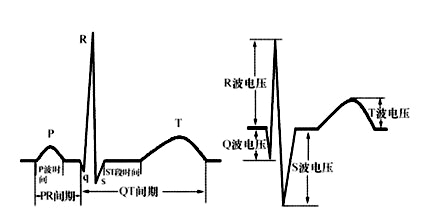
\includegraphics[width=0.6\textwidth]{image2.jpg}
        \caption{心电图各波形、波段示意图}
        \label{F.ECG_image2}
    \end{figure}
    
    本研究针对心电信号采集过程中存在的心电信号幅值微弱、共模噪声干扰以及工频噪声干扰等问题,设计并优化了模拟前端采集电路,包括针对心电信号的放大、滤波与抗干扰措施。此外,为抑制EMI(Electromagnetic Interference)电磁干扰并提高系统的电磁兼容性(Electromagnetic Compatibility, EMC),在电源管理方面特别优化,选型了高开关频率的 DC-DC convert芯片,降低芯片内部 MOS 管开关频率带来的电源噪声。同时在 PCB layout方面,采用模拟和数字电路分区布线,并通过0欧电阻实现单点接地,优化layout设计中对PCB的铜铺和过孔设计,确保模拟信号完整性,减少数字电路和无线射频电路对心电采集电路的干扰。

    \item \textbf{无线通信协议选型}
    
    针对多设备心电数据同步采集的需求,在无线通信协议选型上评估了 Wi-Fi、蓝牙等主流无线通信协议,及其衍生协议如 Wi-Fi Mesh、Bluetooth Mesh等进行选型优化。为选型合适的无线通信协议,对以上所列无线通信协议的设备最大连接数、通信速率、抗干扰能力以及无线环境部署难度进行了实验。本研究在初期开发时验证了多种无线通信协议对心电数据传输的影响,并在协议选型基础上优化网络架构,一定程度提高了数据传输效率,以减少数据包延迟,确保系统可在多设备场景下的稳定运行。针对节点设备的配网、连接及断线重连等环节,设计了基于节点设备MAC地址的节点序设备管理机制,以提高系统的适应性和稳定性。

    \item \textbf{射频性能优化}  
    
    为确保无线射频通信的稳定性与可靠性,本研究对系统的射频特性进行了优化。在射频芯片模组的选型中针对连接天线的射频接口使用了IPEX-1接口,方便更换天线进行测试,同时分析了所购买天线的 S 参数、驻波比(Voltage Standing Wave Ratio, VSWR)及回波损耗(Return Loss)等射频参数,确保天线匹配符合通信需求。

    \item \textbf{多设备数据同步}  
    
    为保证多设备采集数据能够实时重放,无线多设备心电采集系统的开发要点之一是多设备数据的时序同步。由于节点间无法做到同时上电,节点设备间的内置时钟会有巨大差异,将造成各节点所采集的心电数据时间戳不一致的问题。本研究针对该问题,设计了基于时间戳同步和统一时钟同步的策略,各节点通过基站设备构建无线采集网络,并由基站设备授时,建立统一时基,确保各设备异步采集的各数据所打上的时间戳上具有一致性。

    \item \textbf{低功耗优化}  
    
    为实现节点设备的低功耗优化,利用乐鑫公司(Espressif)在ESP32-C3中设计的低功耗特性,通过 Auto Light-Sleep 模式设计系统休眠与唤醒策略。当FreeRTOS进入 空闲任务(IDLE Task)且超过设定的时间阈值后,系统自动进入 Light-Sleep 低功耗休眠模式,以降低功耗。该模式还遵循 DTIM(Delivery Traffic Indication Message)机制,使设备能够在保持 Wi-Fi 连接不断开的同时实现自动的休眠唤醒功能,以确保数据通信的连续性。在此基础上,本研究进一步对系统整体功耗进行了功耗评估与优化,从而有效延长设备的续航时间。

    \item \textbf{上位机系统设计}  
    
    上位机程序为通过QT实现的图形化控制平台,具有设备管理、数据监控、实时心电数据展示及多设备心电数据存储等功能。其通过接收多台节点设备通过UDP发出的心电数据序列帧,将心电数据帧实时反序列化,提取实时心电数据,以提供直观的数据可视化界面,并将心电信号以波形形式展示于用户界面,便于研究人员实时监测受试者的心电状态。以满足实时心电信号监测与存储的需求。
    此外,用户可在上位机程序中灵活配置采集设备的数量,系统支持心电采集节点设备的数量管理,能够根据实际需求人为调整系统的工作规模,以适应不同应用场景。
    为进一步提高数据利用价值,上位机程序具备数据存储与导出功能。系统可对采集数据进行存档,并按需导出为 \textit{CSV} 文件格式,每条记录以 [时间戳, 电平数据] 形式存储并按节点序号位列排开,以便后续数据分析与医学诊断。
    
\end{enumerate}
本研究通过上述技术优化,实现了高效、低功耗、稳定的无线 ECG 多设备同步采集系统。

\subsection{论文组织结构}

全文内容共七章,具体内容组织如下:

第一章为绪论。介绍本文的研究背景以及研究意义,对无线心电同步采集技术的国内外研究现状进行梳理与阐述,最后对本文的研究内容与文章结构进行简要概述。

第二章为心电采集的基础理论部分。介绍心电信号的产生原理以及心电信号中P、Q、R、S、T等波形在心电图中的特点,对心电信号的采集、处理等技术进行详细介绍。

第三章为系统总体设计概述,主要介绍了无线多设备心电同步采集系统的总体设计思路。

第四章为采集系统在硬件部分的设计与实现。主要介绍了心电采集的前端硬件设计思路及原理图设计、心电数据处理和发送的主控部分器件选型思路以及原理图设计、天线选型及射频性能调优过程、整板功耗测量实验数据以及功耗优化策略等硬件相关的技术要点。

第五章为采集系统在嵌入式软件部分的设计与实现。主要介绍了系统的软件架构设计、各节点与主机的时序同步策略、节点所采集的心电数据序列化发送策略、低功耗优化策略等软件相关的技术要点。

第六章为采集系统在上位机软件部分的设计与实现。主要介绍了上位机程序的功能设计、数据接收与解析、数据存储与导出、用户界面设计等上位机软件相关的技术要点。

第七章总结与展望,总结了本文的主要工作,展望了下一阶段的研究方向。

\newpage    % 两个章节之间分页,不想分的话可注释掉

\section{相关背景理论知识}

\subsection{心电信号产生原理}

心电信号是一种反映心脏电活动的生物电信号,其产生源于心肌细胞膜内外离子的流动,主要涉及钠离子(Na$^+$)、钾离子(K$^+$)和钙离子(Ca$^{2+}$)的跨膜转运行为。心脏的正常电活动由心脏传导系统控制,使得心脏各腔室按照一定顺序进行兴奋和收缩,从而完成泵血功能。

在正常的生理状态下,心脏电活动由窦房结(Sinoatrial Node, SA Node)自动发放的兴奋信号起始,并沿特定的传导路径依次传播至心房和心室,完成整个心动周期。具体而言,窦房结所产生的兴奋首先传导至右心房,引发右心房的去极化与收缩;同时,兴奋通过房间束(Bachmann’s Bundle)传至左心房,导致左心房同步收缩。随后,兴奋沿结间束(Internodal Pathways)传至房室结(Atrioventricular Node)。房室结对兴奋信号产生生理性延迟,以确保心房在心室收缩前充分收缩并完成血液充盈。

兴奋通过房室束(Bundle of His)进入心室传导系统,并沿左、右束支(Left and Right Bundle Branches)迅速传递至浦肯野纤维(Purkinje Fibers),最终激活心室肌,导致心室的去极化和收缩。由于心房与心室之间具有特殊的传导路径,这种传导机制确保兴奋能够在短时间内同步传播至心室各部分,从而实现高效的心脏泵血功能。心脏传导模式如图 \ref{F.ECG_image3} 所示 \cite{现代医学电子仪器原理与设计} 。

\begin{figure}[hbt]
    \centering
    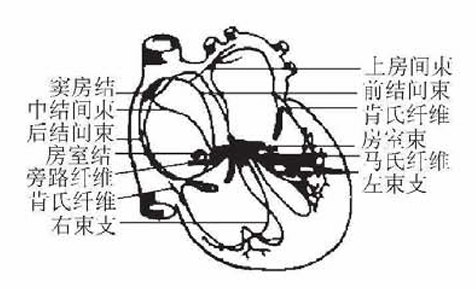
\includegraphics[width=0.6\textwidth]{image3.png}
    \caption{心脏传导系统示意图}
    \label{F.ECG_image3}
\end{figure}

在每一个心动周期中,心脏各部位依照一定的顺序和时间规律经历兴奋的产生、传播和恢复,其电活动表现出方向性、时间性及空间上的特定规律。这些生物电信号可通过心脏周围的导电组织和体液传导至体表,使人体不同部位在每个心动周期中均发生相应的电位变化。心电图(Electrocardiogram, ECG)即是在人体表面特定位置放置电极,以记录这些电信号变化的曲线。心电图能够全面反映心脏兴奋的产生、传导及复极化过程,为心脏功能的评估和疾病诊断提供重要依据。

\subsection{心电图波形特征}

\begin{figure}[hbt]
    \centering
    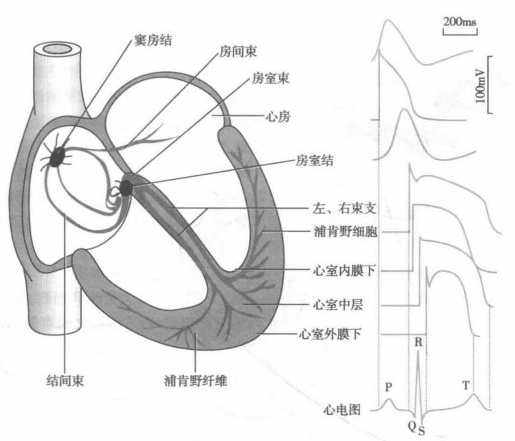
\includegraphics[width=0.6\textwidth]{image4.png}
    \caption{心电图形成示意图}
    \label{F.ECG_image4}
\end{figure}

如图 \ref{F.ECG_image4} 所示 \cite{人体解剖生理学} 心电图(Electrocardiogram, ECG)波形的变化反映了心脏不同阶段的电生理活动。典型的心电图波形包括 P 波、QRS 复合波、T 波和 U 波,如图\ref{F.ECG_image5}所示 \cite{现代医学电子仪器原理与设计} ,各波形的生理意义和正常范围如下:

\begin{enumerate}
    \item \textbf{P波}:P 波由心房去极化产生,其前半部分主要由右心房去极化形成,后半部分主要由左心房去极化形成。正常情况下,P 波的持续时间不超过 0.10 s。

    \item \textbf{P-R间期}:P-R 间期是指 P 波起点到 QRS 复合波起点之间的时间间隔,代表从心房开始兴奋到心室兴奋的时间,即兴奋通过心房、房室结和房室束的传导时间。P-R 间期会随着年龄增长而呈现轻微延长的趋势。

    \item \textbf{QRS复合波}:QRS 复合波反映了左、右心室的去极化过程。QRS 波群的持续时间称为 QRS 时限,代表整个心室肌去极化过程所需的时间。正常情况下,QRS 时限不超过 0.10 s。
    
    \item \textbf{S-T段}:S-T 段是指 QRS 复合波终点到 T 波起点之间的时间区间,代表心室肌复极化的缓慢阶段。正常情况下,该段接近基线,其与基线的偏离一般不超过 0.05 mm。

    \item \textbf{T波}:T 波代表心室肌的复极化过程。在 R 波占主导的心电图中,T 波的幅值应不低于 R 波幅值的 1/10。

    \item \textbf{U波}:U 波出现在 T 波之后,相对基线来说是凹陷的波形,与心室肌复极化后的电位变化相关。
\end{enumerate}

\begin{figure}[hbt]
    \centering
    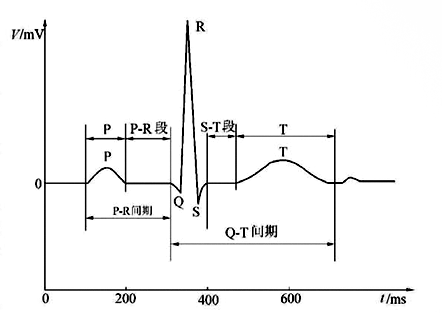
\includegraphics[width=0.6\textwidth]{image5.png}
    \caption{心电图各波段示意图}
    \label{F.ECG_image5}
\end{figure}

\subsection{心电信号采集原理}
在人体体表进行心电图(ECG)记录时,需要解决两个核心问题:一是如何确定电极的放置位置,以确保获得稳定且具有临床价值的信号;二是如何设计电极与放大器的连接方式,以保证信号的准确传输和放大。

\subsubsection{心电图导联方式}

为了实现心电图波形的标准化,提高数据的可比性和诊断的可靠性,临床实践中对电极的放置部位及其连接方式进行了严格规范。按照心电图学的专业术语,电极在人体体表的具体放置方式以及其与放大器的连接形式统称为心电图导联。

心电图导联主要分为标准导联和非标准导联两大类。标准导联是指按照国际标准规定的电极放置位置和连接方式进行心电图记录,包括 I、II、III等导联形式。

标准导联中I、II、III导联由Einthoven发现,是最早的心电图导联,其原理是利用三个电极在人体体表上的不同位置记录心电信号,以反映心脏的不同方向的电活动。这三个导联的电极放置位置如图\ref{F.ECG_image6}所示 \cite{现代医学电子仪器原理与设计} 。其中,I导联的电极放置在左右手腕,II导联的电极放置在右手腕和左脚踝,III导联的电极放置在左手腕和左脚踝。

\begin{figure}[hbt]
    \centering
    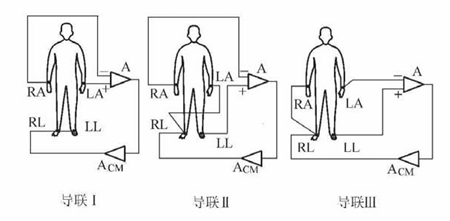
\includegraphics[width=0.6\textwidth]{image6.png}
    \caption{I、II、III导联电极放置示意图}
    \label{F.ECG_image6}
\end{figure}

\subsubsection{心电信号放大与滤波}

心电信号的幅值一般在 0.5 mV 至 5 mV 之间,在采集与传播途中容易夹杂人体产生的共模噪声以及周围电器的市电工频噪声,具有较低的信噪比。为了保证心电信号的准确采集和分析,需要对信号进行适当的放大和滤波处理。最早的心电图机采用机械放大器和滤波器,通过机械装置调节放大倍数和滤波频率,实现对心电信号的处理。随着电子技术的发展,现代心电图机采用电子放大器和滤波器,通过电子元件实现对心电信号的放大和滤波。如图\ref{F.ECG_image7} a,b所示 \cite{现代医学电子仪器原理与设计} ,两种方式的采集前端基本相同,均由电极、放大器和滤波器组成。

\begin{figure}[H]
    \centering
    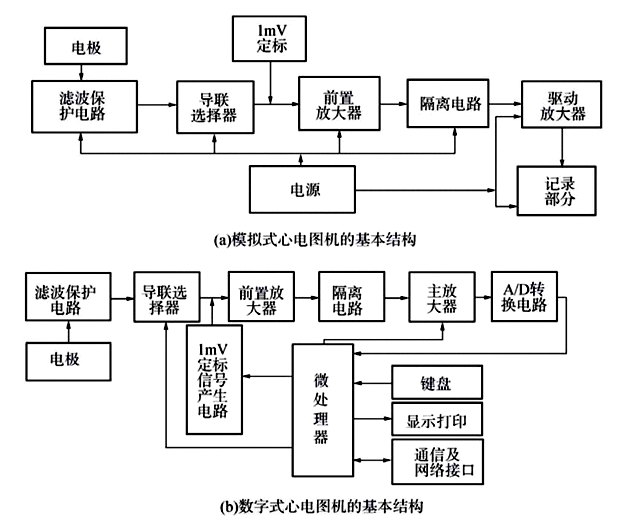
\includegraphics[width=0.8\textwidth]{image7.png}
    \caption{心电信号放大与滤波原理图}
    \label{F.ECG_image7}
\end{figure}

心电信号输入部分包括电极、导联线和前置放大器,其中电极用于接触人体体表,导联线用于传输心电信号。导联线作用是从人体中提取原始的心电信号,并按照导联组合,将信号传输至放大器。导联线将电极片上采集到的心电信号传递到前置放大器,前置放大器对信号进行放大和滤波处理。采取I、II、III导联的话导联线一般是6根,但根据实际使用的话一般只需要使用3根导联线即可完成一种导联的连接。导联线如图\ref{F.ECG_image8}所示,其中红色线为右手腕电极符号为RA或R,黄色线为左手腕电极符号为LA或L,绿色线为左腿电极。

\begin{figure}[hbt]
    \centering
    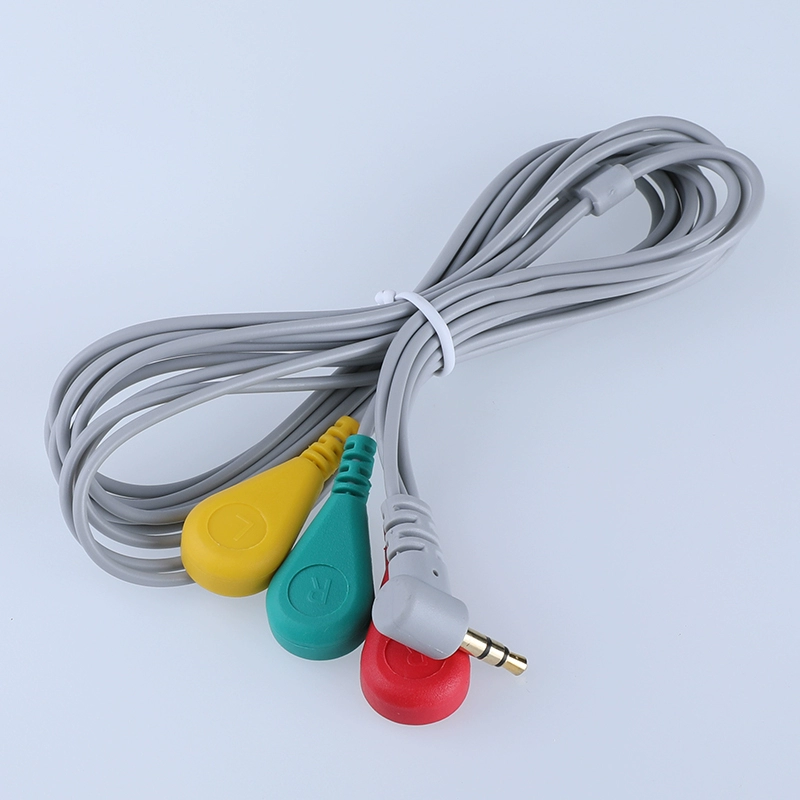
\includegraphics[width=0.4\textwidth]{image8.png}
    \caption{心电采集导联线示意图}
    \label{F.ECG_image8}
\end{figure}

在心电信号的采集与处理过程中,对信号进行滤波放大的模拟前端起着至关重要的作用。由于人体心电信号的幅度通常处于毫伏(mV)级别,信号较为微弱,且容易受到外界电磁干扰和生理噪声的影响,因此,在信号进入后续处理单元之前,需通过模拟前端进行初步的放大滤波,以提高信号的幅值和信噪比,确保后续采集的准确性和稳定性。

前端放大器的主要功能在于将电极采集到的原始心电信号放大至合适的幅度,使其能够满足后续滤波、模数转换(A/D 变换)及数据采集的要求。合理设计的前端放大器不仅应具备高增益特性,还应具有较低的噪声、优良的共模抑制比(CMRR)以及适当的输入阻抗,减少回波反射和信号失真,确保信号的准确采集和传输。心电信号是差模信号,因此前端放大器一般会先通过差分信号放大器突出心电信号的差模成分并移植共模噪声干扰,同时将共模信号通过右腿驱动电路反相放大后输入人体,抵消人体的共模噪声。再通过仪表放大器芯片进行前置放大,提高心电信号的幅值,以便后续的滤波和模数转换。

心电信号中噪声干扰一般是来自于市电工频干扰、人体肌肉电信号干扰、基线漂移等,这些问题会对心电信号的采集和分析造成影响。为了减少这些干扰信号对心电信号的影响,需要对心电信号进行滤波处理。滤波器的作用是通过对心电信号进行滤波,去除掉不需要的频率成分,保留需要的频率成分。心电采集中常用的滤波器有低通滤波器、高通滤波器以及陷波滤波器。低通滤波器的作用主要是去除板级DC-DC电源模块的开关频率带来的电源噪声,高通滤波器的作用主要是去除肌电干扰,肌电干扰是由人体肌肉带动肢体运动产生的不规则高频电干扰,其频率一般在10-1000Hz之间,通过高通滤波器可以去除这部分干扰信号并且可以消除基线漂移。陷波滤波器的作用是滤除特定频率的波形,在心电采集中的作用是去除50Hz市电工频的干扰。

最后通过放大和滤波的心电信号由MCU进行模数转换,将模拟信号转换为数字信号,以便后续的数据处理和存储。

\newpage    % 两个章节之间分页,不想分的话可注释掉


\section{系统各部分设计概述}

本系统由心电采集节点设备、基站设备及上位机软件三部分组成,以实现多设备同步的心电信号采集存储系统。本研究成功实现了在局域网环境下较大规模心电采集设备的低延迟、高频率同步采集功能,同时确保了多个心电采集节点间的时序同步。

系统支持 10 个及以上的心电采集设备,并通过基站提供的全局时钟基准,实现不同受试者心电信号的时间同步。各采集节点依据基站发送的时间同步偏移量进行调整,确保所有数据的时间戳一致,从而保证各节点设备在协同工作时能够同步采集。每个心电采集节点的采样速率可达 1000 Hz,能够以毫秒(ms)级记录心电信号的细微变化,同时通过WiFi与上位机建立socket连接,通过UDP发送序列化的数据包,使系统在保证高数据率的同时满足实时性要求。

采集系统还配备上位机控制与监测软件,支持灵活配置采集设备数量,满足不同实验环境与应用需求,并具备实时显示心电波形的功能,能够为用户提供直观的实时监看界面。上位机还支持数据存储与导出,便于后续信号分析。如图\ref{F.ECG_image9}所示,为系统的功能设计框图。

通过ESP-TOUCH的配网技术以及面向无连接的ESP-NOW通信技术,采集系统能够在不同的网络环境下自动组网,快速部署,并基于无线通信技术降低布线复杂度,提升部署的灵活性和适应性,使其在实验室、医疗机构及远程监测等场景中均能高效、准确地完成心电信号采集。

\begin{figure}[hbt]
    \centering
    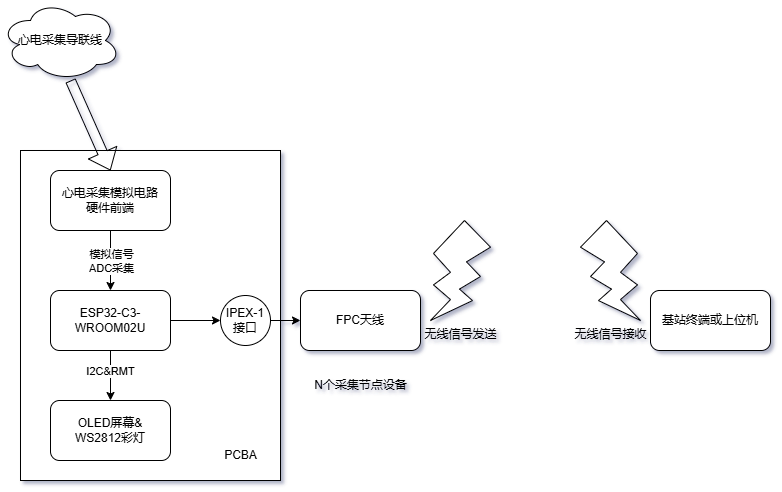
\includegraphics[width=0.8\textwidth]{image9.png}
    \caption{系统功能设计框图}
    \label{F.ECG_image9}
\end{figure}

\subsection{心电采集与发送的节点设备}

本设备主要承担心电信号的获取、初步数据处理及数据传输功能,确保心电信号的高质量采集与可靠传输。设备采用单导联心电信号采集方式,通过电极片获取人体生物电信号,并将信号引入板载 3.5mm 耳机接口,经由心电信号采集模拟前端电路进行信号调理,以满足后续数据处理的需求。

在信号处理方面,心电信号首先经过仪表放大芯片以提升信号幅度,并将共模噪声通过右腿驱动电路注入回人体,随后通过滤波电路进行噪声抑制。其中,低通滤波用于去除高频干扰,避免外部电磁干扰对心电波形的影响,而带阻滤波主要针对 50Hz 工频噪声进行抑制,以降低电网干扰对信号的影响。在完成模拟信号的预处理后,信号通过主控芯片ESP32-C3的ADC部分采集处理发送。设备支持理论最高 1000 Hz 采样率,能够精准捕获心电信号的动态变化,以满足数据分析的需求。

\subsection{时钟同步与组网的基站设备}

基站设备在系统中的主要任务是为各节点采集设备提供基准时钟信号,使系统内的各个采集节点能够按照统一的时间基准对所采数据打上时间戳,从而确保不同节点设备之间的心电数据时间对齐。在时间同步方面,基站设备利用 ESP-NOW 无线通信协议,在各节点设备通过配网加入采集网络时,向每个新连接的节点提供本机的时间。节点设备接收到基准时间后,调整自身的本地时钟偏移量。这一同步机制可有效降低了多设备数据融合时的时间误差。

除了时间同步功能,基站设备还负责对整个网络中的设备进行状态监控。基站能够实时显示当前已连接的心电采集设备数量,并提供上位机所在主机的IP 地址、WiFi 连接情况等关键信息,便于系统监测和维护。

\subsection{数据接收与监控的上位机软件}

上位机程序通过pyQT实现了图形化的用户界面,提供了设备管理、实时心电数据展示及心电数据存储等功能。

在数据通信方面,上位机程序通过Socket建立实时数据接收通道,以UDP方式接收各心电采集节点发送的序列化心电数据包,并基于心电信号的时间戳信息进行数据反序列化,并将数据按时间与电压幅值进行可视化。采集到的数据以心电图波形的形式通过QT的matplot绘图功能将数据实时呈现在用户界面上,使研究人员能够直观监看受试者的心电信号状态。

上位机程序支持节点设备数目的管理与配置,用户可根据实际需求调整节点采集设备的数量,实现对不同实验条件或应用场景的适配。系统允许在测量开始前人为添加或移除采集设备,并提供设备状态监控功能,以确保所有节点均处于正常工作状态。 

上位机程序具备数据存储与导出功能,可对采集的心电数据导出为CSV文件,数据格式为 [时间戳, 放大后的心电信号幅值],以便后续的信号分析与医学诊断。该功能确保心电数据的长期可用性,使研究人员能够在不同时间点对数据进行回溯与深入分析。

\subsection{系统灵活性与易用性设计}

为了满足不同应用场景的需求,本研究在系统的灵活性和易用性上,为确保设备在多变的应用环境下能够快速部署,并便捷地进行配置和调整。采集系统在设计上兼顾了可扩展性、图形化管理以及动态数据采集存储,确保多设备协同工作时的稳定性和可靠性。以下是系统在灵活性方面的主要设计特点。

在实际应用中,心电采集设备可能分布于不同地点,且所需的设备数量随应用需求变化而不固定。因此,本系统支持动态调整采集设备的数量,用户可以根据需求自由增减设备,而无需对系统架构进行大幅修改,也无需重新编译或烧录固件,从而提高了系统的适应性和可扩展性。为简化设备的网络配置,系统支持ESP-TOUCH智能配网方案,用户可通过 ESP-TOUCH 手机应用快速完成基站的 Wi-Fi 配置。只需在手机 APP 中输入 Wi-Fi 的名称和密码,基站便可自动连接至指定网络,实现一键式配网,极大地降低了设备部署的复杂性。如图\ref{F.ECG_image10}所示,为ESP-TOUCH示意图。

\begin{figure}[hbt]
    \centering
    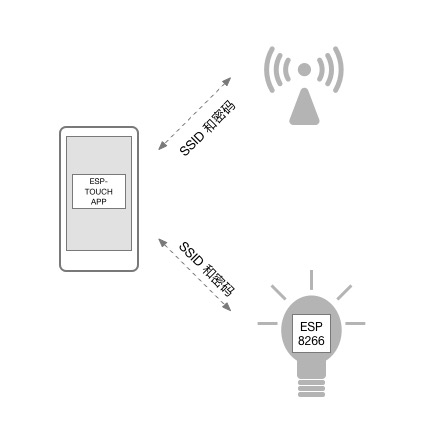
\includegraphics[width=0.6\textwidth]{image10.jpg}
    \caption{ESPTOUCH配网示意图}
    \label{F.ECG_image10}
\end{figure}

系统采用自动组网机制,节点设备与基站设备通过局域网进行无线连接。节点设备无固定编号,节点编号由基站根据设备上电顺序进行动态分配,从而避免了编号管理的繁琐操作,节点设备的接入顺序对系统运行无影响。

每个节点设备在启动时,会自动向基站发送连接请求,并在接入网络后根据基站提供的全局时钟信号调整自身的时间基准,以保证在不同时间上电的采集设备能够时间同步。即使系统中设备数量发生变化,或部分设备掉线,基站仍可维持工作,使得新加入或重新连接的节点能够无缝接入,继续采集心电数据,而无需重启整个系统或重新组网。通过此种设计提高系统的稳定性和容错能力。

由于节点设备的启动顺序不受限制,用户可随时启用或关闭任意节点,而无需预先进行设备排序或额外的手动同步操作。基站在检测到新节点接入时,会自动完成时间同步和编号分配,确保该节点能够在当前系统时钟下继续记录数据,而不会影响其他设备的正常采集过程。

\newpage    % 两个章节之间分页,不想分的话可注释掉

\section{主要硬件部分设计与实现}

\subsection{心电信号采集节点硬件原理图设计}

\subsubsection{主控MCU部分}

主控单元选用乐鑫信息科技(Espressif Systems)推出的ESP32-C3-WROOM-02低功耗无线SoC模组,该芯片集成RISC-V架构32位单核处理器(最高时钟频率160MHz)与2.4GHz无线通信子系统。系统通过其内置的12位高精度SAR型ADC模块(可配置采样率范围4kHz-40kHz)对前端模拟信号处理电路输出的差分心电信号进行数字化转换。模组内建的IEEE 802.11b/g/n Wi-Fi 4协议栈,支持2.4GHz频段的无线通信,可实现与上位机的数据传输。此外,ESP32-C3还集成了丰富的外设接口,包括SPI、I2C、UART、PWM、ADC等,方便与外部传感器、存储器等设备进行通信。

在本系统中节点设备使用了ESP32C3的高精度ADC功能,对心电信号进行模数转换和电池电压采集,并通过芯片内的WiFi基带将心电数据通过2.4GHz频段的无线WiFi网络将心电数据发送至上位机。同时,通过芯片的RMT(Remote Control Transceiver)功能控制板载WS2812的颜色及闪烁频率,实现设备状态的指示。并预留I2C接口,方便后续扩展其他传感器模块,如与血氧测量芯片通信,实现多参数生理信号采集。

为优化开发流程,设计基于沁恒微电子CH343G高速USB-UART桥接芯片的自动下载电路。该电路通过解析上位机通过串口发送的DTR(Data Terminal Ready)和RTS(Request To Send)控制信号,配合RC延时网络(典型值:R=10kΩ,C=100nF)生成符合ESP32-C3启动模式要求的时序组合,并人为切换从Joint Download Boot模式或SPI Boot模式启动,如表\ref{T.ESP32C3-startmode}所示为ESP32C3各启动模式的配置表。此时通过原理图设计,将GPIO2和GPIO8上拉后只需要控制GPIO9的电平即可实现两种启动模式的切换。在ESP32C3的定义中GPIO2、GPIO8、GPIO9都为Strapping Pin,通过控制这三个管脚的电平即可实现不同启动模式的切换。

\begin{table}[htb]
    \centering
    \caption{ESP32-C3启动模式表}
    \label{T.ESP32C3-startmode}
    \begin{tabular}{llll}
    \hline
    启动模式 & GPIO2 & GPIO8 & GPIO9 \\
    \hline
    SPI Boot (default) & 1 & 任意值 & 1 \\
    \hline
    Joint Download Boot & 1 & 1 & 0 \\
    \hline
\end{tabular}
\end{table}

如表\ref{T.ESP32C3-autodownload}所示为ESP32C3自动下载电路的真值表。按照乐鑫官方技术文档\cite{espressif2021esp32c3}可知EN的为电平为0即低电平时芯片关闭,EN为1即高电平时芯片启动。通过控制DTR输出1,RTS输出0,此时GPIO9为1,EN为0,将芯片关闭,延时100ms,再将DTR输出为0,此时EN理应为1,GPIO9为1,芯片启动,不延时立刻将RTS输出为1,此时GPIO9为0,在此刻由于芯片EN脚接入了一个RC延时网络,EN并不会立刻上升为高电平,而是会缓慢上升,当EN的电平上升至0.75的VDD时,芯片启动,此时由于GPIO9的电平为0,芯片进入Joint Download Boot模式。延时50ms将GPIO9这个Strapping Pin维持超过芯片的保持时间$t_H$(如图\ref{F.ECG_image13}所示),等芯片读取完Strapping管脚的电平后再将RTS输出为1,此时EN为1,GPIO9为1,当完成下载并复位芯片时,芯片能够正确从SPI Flash中启动用户代码。通过上述真值表的设计,实现了自动下载电路的功能,方便用户快速烧录固件。

\begin{table}[htb]
    \centering
    \caption{自动下载电路真值表}
    \label{T.ESP32C3-autodownload}
    \begin{tabular}{llllll}
    \hline
    DTR & RTS & EN & GPIO9 \\
    \hline
    0 & 0 & 1 & 1 \\
    \hline
    0 & 1 & 1 & 0 \\
    \hline
    1 & 0 & 0 & 1 \\
    \hline
    1 & 1 & 1 & 1 \\
    \hline
\end{tabular}
\end{table}

\begin{table}[htb]
    \centering
    \caption{Strapping 管脚的时序参数说明}
    \label{T.ESP32C3-strapping}
    \begin{tabular}{|l| p{8cm} |r|} % 3列:左对齐、左对齐、右对齐
    \hline
    \textbf{参数} & \textbf{说明} & \textbf{最小值(ms)} \\
    \hline
    $t_{\mathrm{SU}}$ & 建立时间:拉高 CHIP\_EN 激活芯片前,电源轨达到稳定所需时间 & 0 \\
    \hline
    $t_{\mathrm{H}}$ & 保持时间:CHIP\_EN 已拉高后,strapping 管脚变为
    
    普通 IO 前可读取其值的时间 & 3 \\
    \hline
    \end{tabular}
\end{table}

\begin{figure}[H]
    \centering
    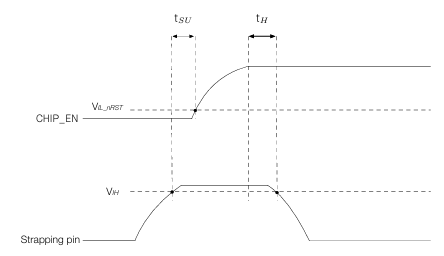
\includegraphics[width=0.6\textwidth]{image13.png}
    \caption{Strapping 管脚时序参数图}
    \label{F.ECG_image13}
\end{figure}

\begin{figure}[hbt]%不知道为什么这个图插入到下一段底下就会报错,只能插入在这里
    \centering
    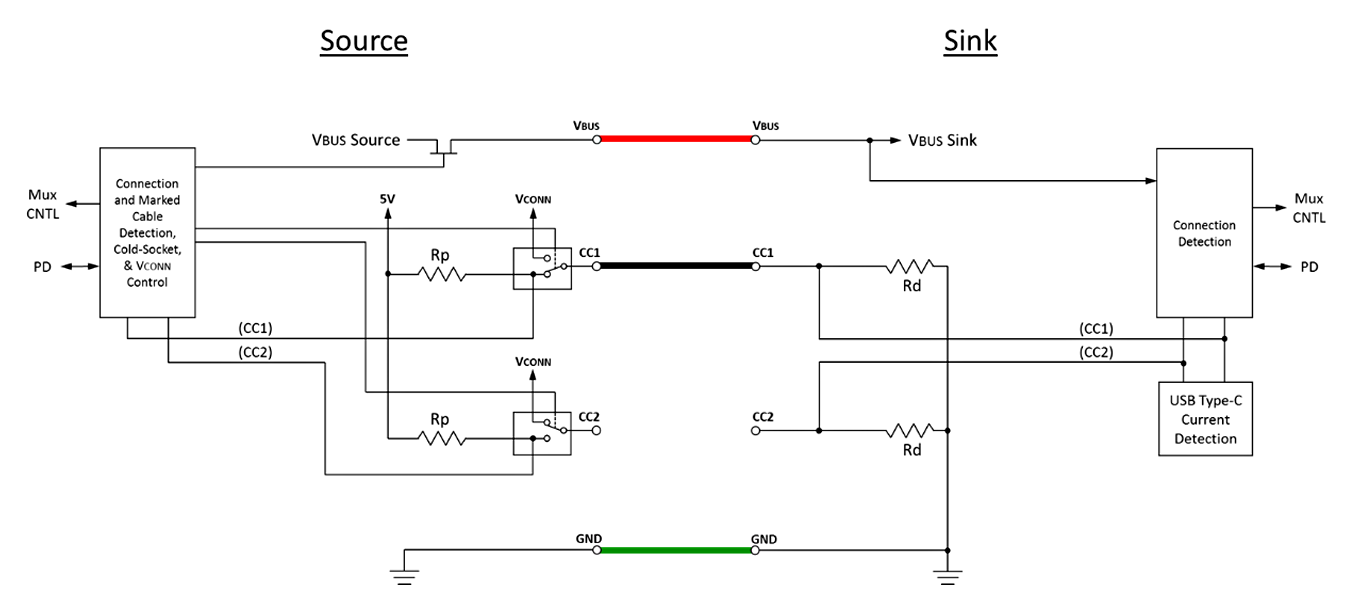
\includegraphics[width=1\textwidth]{image14.png}
    \caption{供电源到Sink设备的功能模式图}
    \label{F.ECG_image14}
\end{figure}

设备采用USB Type-C接口作为标准供电端口,遵循Type-C® Cable and Connector Specification Release 2.4规范。如图\ref{F.ECG_image14} \cite{usbtypec24}所示,在设备端接口CC1、CC2引脚与地之间各配置5.1kΩ±1$\%$精度电阻,形成Rp=5.1kΩ的固定下拉配置,向供电端明确声明本设备作为Sink设备的功率需求等级可向供电设备申请5V/3A的输入到设备中。使得通过C to C线材接入电脑进行调试的同时能够为板载锂电池充电,而避免产生接入后由于Type-C协议不匹配导致无法为设备供电的问题。

本设计通过上述关键技术点的实现,构建了符合医疗电子设备基本要求的硬件平台,其模块化架构便于后续功能扩展与性能优化。如图\ref{F.ECG_image11}所示,为心电信号采集节点硬件原理图设计。

\begin{sidewaysfigure}
    \centering
    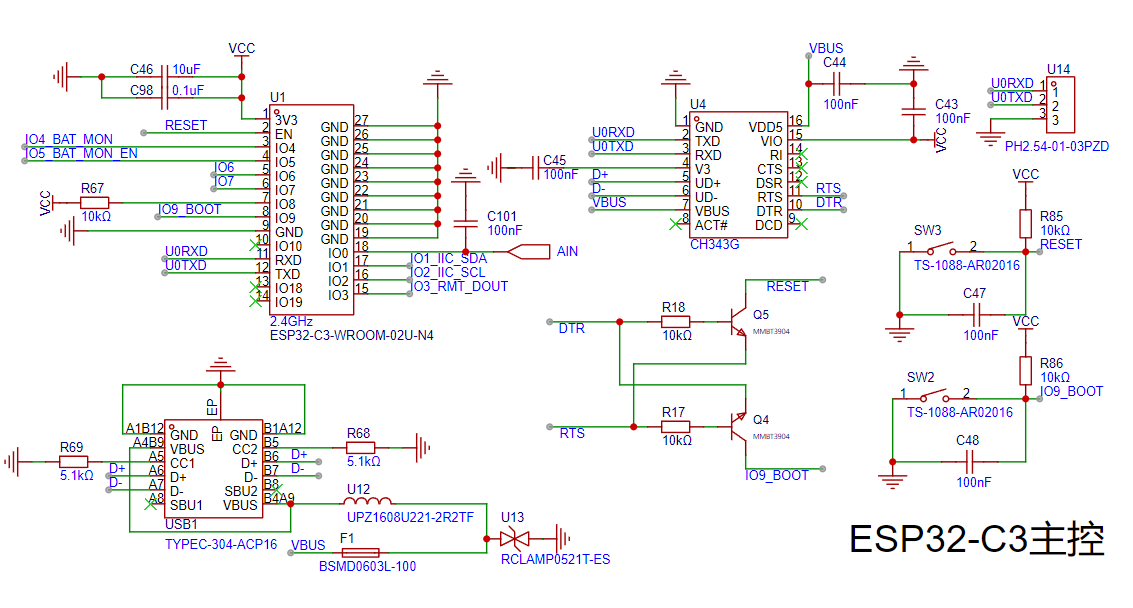
\includegraphics[width=1\textwidth]{image11.png}
    \caption{心电信号采集节点主控部分硬件原理图设计}
    \label{F.ECG_image11}
\end{sidewaysfigure}

\newpage    % 两个章节之间分页

\subsubsection{电源部分}

节点设备在电源部分采用三级供电架构设计,重点解决锂电池安全保护、多电压域转换以及供电模式切换可靠性等技术问题。

在锂电池保护电路设计中,为避免锂电池因过充电、过放电、电流过大导致电池寿命衰减或电池被损坏,使用杰盛微(JSMICRO)DW01锂电保护芯片,配合双NMOS管FS8205A组成标准保护电路。当检测到电池电压超过过充阈值(典型值4.35V±25mV)或低于过放阈值(2.4V±50mV)时,芯片通过内部比较器触发OC/OD引脚电平翻转,切断MOS管通路实现硬件级保护。该电路设置100ms的延时响应时间,可有效过滤瞬态电压波动导致的误触发。

设备采用了TP5400作为锂电池的充放电管理芯片。TP5400 为一款移动电源专用的单节锂离子电池充电器和恒定5V升压控制器,充电部分集高精度电压和充电电流调节器、预充、充电状态指示和充电截止等功能于一体,可以输出最大1A充电电流。而升压电路采用CMOS工艺制造的空载电流极低的VFM开关型DC/DC升压转换器。其具有极低的空载功耗(小于10uA),且升压输出驱动电流能力能达到1A。充电部分为线性降压方式,内置PMOSFET,加上防倒灌电路,并不需要外部检测电阻器和隔离二极管。热反馈可对充电电流进行自动调节,以便在大功率操作或高环境温度条件下对芯片温度加以限制,充满电压固定于4.2V。充电电流可通过一个电阻器进行外部设置。当电池达到4.2V之后,充电电流逐渐下降至设定电流值的五分之一,TP5400将自动终止充电,如图\ref{F.ECG_image15}为TP5400在为1000mAh电池充电的数据图\cite{TP5400}。TP5400对充电温度保护方面也集成了相关的保护功能,可根据输出负载情况动态调节电流。 同时TP5400还可接入两颗LED灯,分别用于充电中指示和充电完成指示。

\begin{figure}[hbt]
    \centering
    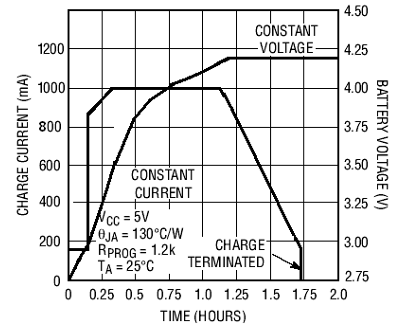
\includegraphics[width=0.6\textwidth]{image15.png}
    \caption{TP5400充电循环图(1000mAh电池)}
    \label{F.ECG_image15}
\end{figure}

由于TP5400在进行锂电池充电时升压部分无法工作,因此在电池充电时,节点设备需要通过TYPE-C接口进行供电。因此节点设备在电源设计中设计了电源自动切换电路,可在接入TYPE-C充电时自动切换为外部供电模式,而在拔掉TYPE-C充电线时自动切换为锂电池供电模式。通过MOS管Q1和Q2的控制,实现了电源的自动切换。当TYPE-C充电线接入时,VBUS通过肖特基二极管D10输入到VCC5V中,此时VBAT5V为0V,但是D11截止了VBUS倒灌至电池,当TYPE-C拔除后,VBUS电压为0V,VCC5V由VBAT5V供电,实现了电源的自动切换。如图\ref{F.ECG_image19}所示为电源切换电路原理图。

\begin{figure}[hbt]
    \centering
    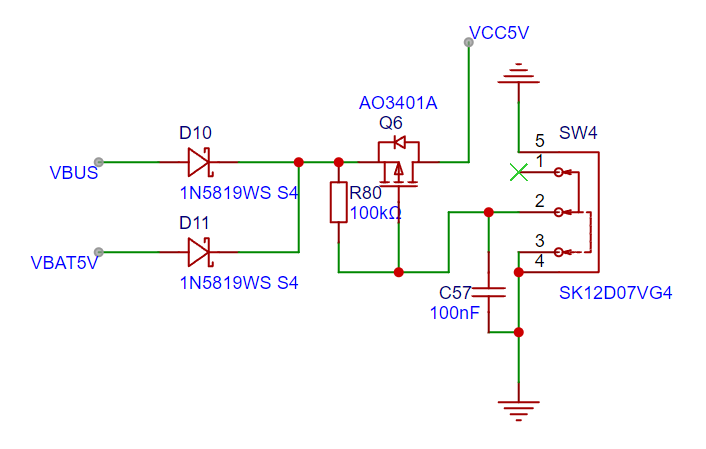
\includegraphics[width=0.6\textwidth]{image19.png}
    \caption{电源切换电路原理图}
    \label{F.ECG_image19}
\end{figure}

由于电池通过TP5400升压后输出的电压为5V,以及在充电时由USB进行供电的电压也是5V,因此在节点设备中需要将5V电压转换为3.3V电压,以满足主控芯片、传感器等模拟电路的工作电压要求。将锂电池的5V电压域转换为芯片工作的3.3V电压域的设计中,采用了矽力杰(Silergy)SY8088IAAC 同步降压DC/DC稳压器实现5V→3.3V的转换。SY8088I是一款高效率的1.5MHz同步降压DC/DC稳压器,能够提供高达1A的输出电流。它可以在2.5V至5.5V的宽输入电压范围内工作,并集成了主开关和同步开关,具有非常低的导通电阻(RDS(ON)),以最大限度地减少导通损耗。1.5MHz的开关频率实现了低输出电压纹波,并使外部电感器和电容器的尺寸得以减小。如图\ref{F.ECG_image16}为SY8088I的应用电路图,通过电容电感实现Buck电路降压输出,控制输入SY8088I的反馈引脚的电压,可以实现LX引脚输出电压的调节,从而满足不同电路的工作电压需求。

\begin{figure}[hbt]
    \centering
    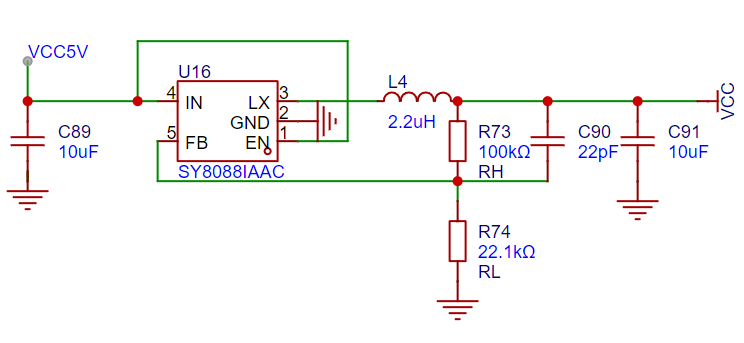
\includegraphics[width=0.6\textwidth]{image16.png}
    \caption{SY8088I应用电路图}
    \label{F.ECG_image16}
\end{figure}

通过查阅SY8088I的datasheet可知,如图\ref{F.ECG_image17},此芯片通过反馈引脚的输入电压与内置的0.6V参考电压进行比较,来控制LX引脚的电压输出。

\begin{figure}[hbt]
    \centering
    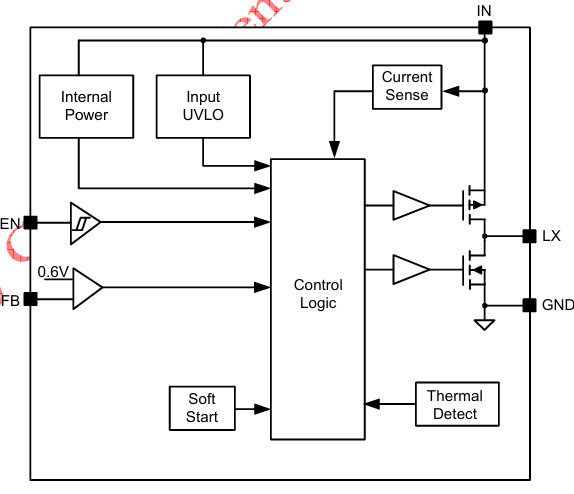
\includegraphics[width=0.6\textwidth]{image17.png}
    \caption{SY8088I功能方框图}
    \label{F.ECG_image17}
\end{figure}

通过电阻分压电路控制反馈引脚的电压,当所需电压固定的情况下,即可计算电阻分压电路所需阻值,公式如\ref{E.SY8088I}所示为SY8088I的输出3.3V电压的计算公式,此处固定电阻分压电路中$R_H$为$100\,\text{k}\Omega$。

\begin{equation}
        V_{\text{out}} = \frac{0.6 \times 100\,\text{k}\Omega}{22.1\,\text{k}\Omega} + 0.6\,\text{V} \approx 3.31\,\text{V}
    \label{E.SY8088I}
\end{equation}

节点设备在电源部分还设计了基于NMOS(AO3400)和PMOS(AO3401A)的隔离式低功耗电池电压测量电路:ESP32-C3 使能电池电压测量的管脚输出高电平时,PMOS管Q8导通,将NMOS管Q7栅极下拉到地,控制其导通,电池电压经电阻分压电路分压一半后输入电池电压测量ADC管脚。此电路的优势在于其在不测量电池电压即PMOS Q8截止时,电路处于断开状态,不会对电池产生额外的负载,降低整板的空载功耗,提升设备运行时间。如图\ref{F.ECG_image18}为电池电压测量电路原理图。

\begin{figure}[hbt]
    \centering
    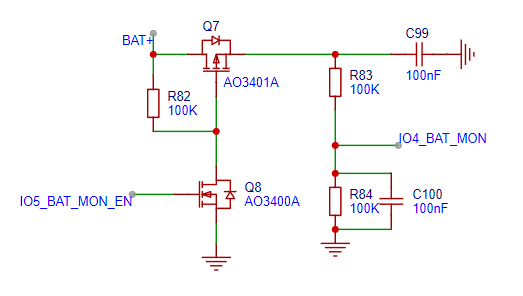
\includegraphics[width=0.6\textwidth]{image18.png}
    \caption{电池电压测量电路设计图}
    \label{F.ECG_image18}
\end{figure}

\begin{sidewaysfigure}
    \centering
    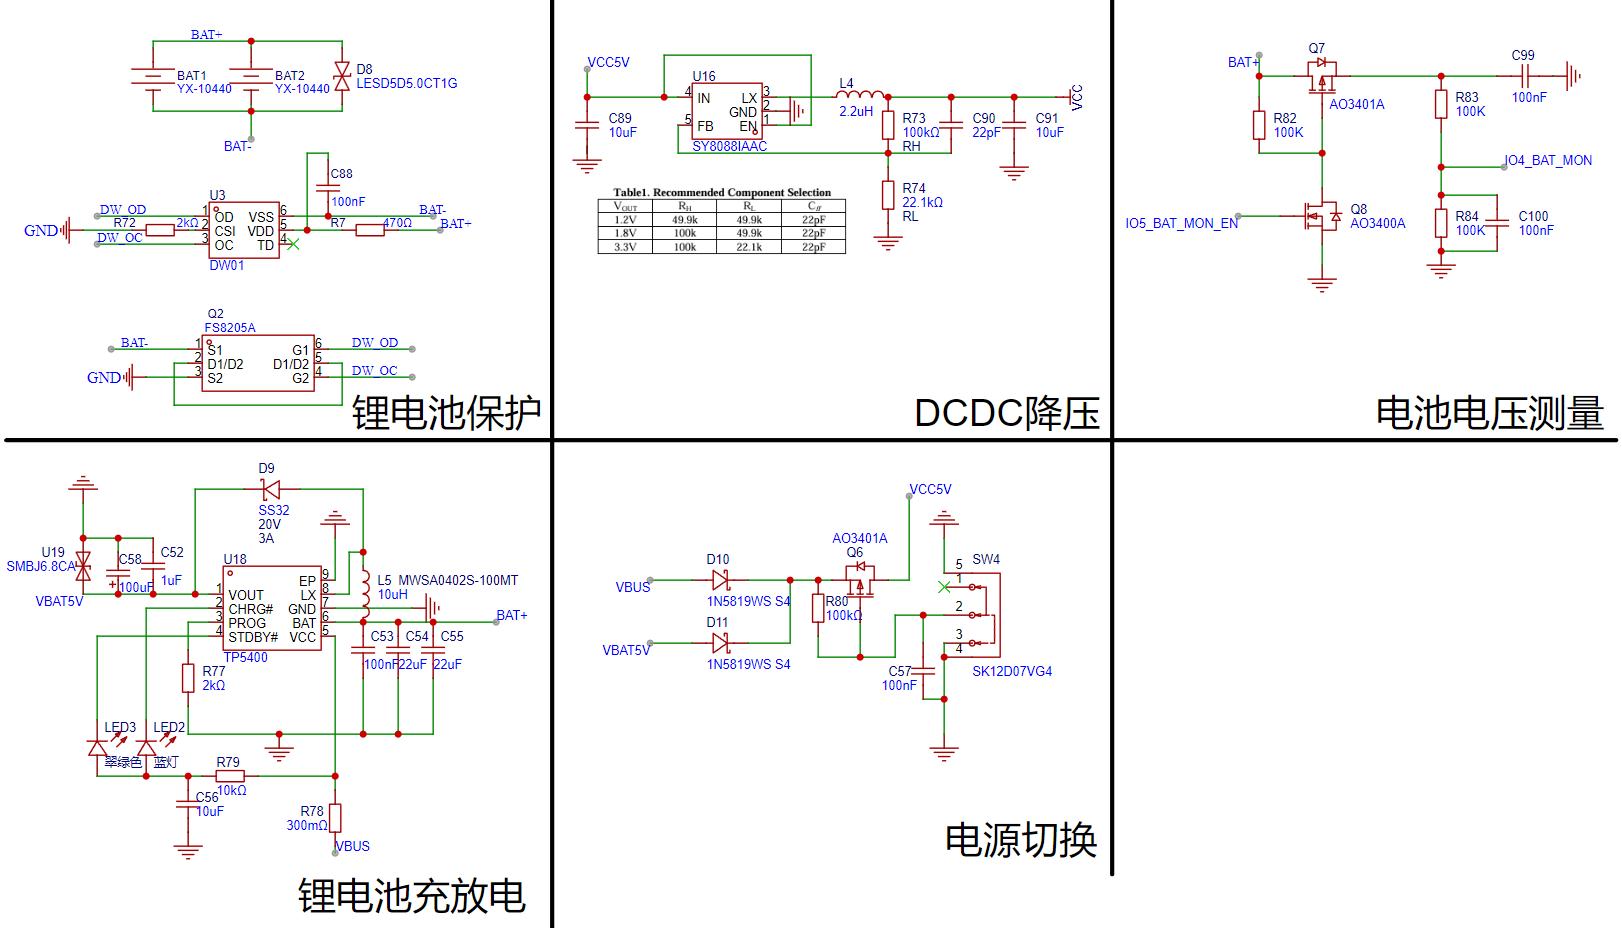
\includegraphics[width=1\textwidth]{image20.png}
    \caption{心电信号采集节点电源部分硬件原理图设计}
    \label{F.ECG_image20}
\end{sidewaysfigure}

\newpage    % 两个章节之间分页

\subsubsection{心电采集与放大部分}

节点设备心电采集与放大部分作为决定心电数据采集质量的核心部分,需通过多级精密调理电路实现微弱生理信号的可靠提取。在设计上由运放电源管理、信号采集、前置放大、共模抑制、噪声滤波和电平适配等环节构成完整的信号处理链路。

在电源架构设计上,系统采用LM2776电荷泵实现双极性供电方案,将3.3V直流电源转换为±3.3V对称电源。该设计有效解决了单电源供电时运算放大器工作范围受限的问题,使运算放大器能够在正负电压下正常工作,避免了单电源供电可能导致的信号失真。为保障电源质量,在电荷泵输出端采用电容滤波处理,包含100nF与两个并联的47μF陶瓷电容滤波器,有效抑制电荷泵开关过程引入的低频纹波噪声,以满足生物电信号采集的低噪声需求。

信号输入通道采用标准三电极导联体系,通过RA(右手)、LA(左手)、RL(右脚) 电极构成威尔逊中心电端。前置调理单元选用AD620A仪表放大器构建差分输入结构,其120dB共模抑制比(CMRR)可有效抑制肢体运动等引入的共模干扰。根据AD620A在ECG测量的典型应用中,如图\ref{F.ECG_image21} \cite{AD620A},首级增益设置为7倍,在保证信号保真度的同时避免放大器饱和。针对体表存在的工频共模干扰,采用右腿驱动负反馈的设计,将AD620A提取的共模电压经LM258DR运放反相放大后通过RL电极反馈至人体,由于反馈信号与原始共模噪声相位相反,当它们在人体中叠加时,能够相互抵消,从而有效降低共模噪声的影响。

\begin{figure}[H]
    \centering
    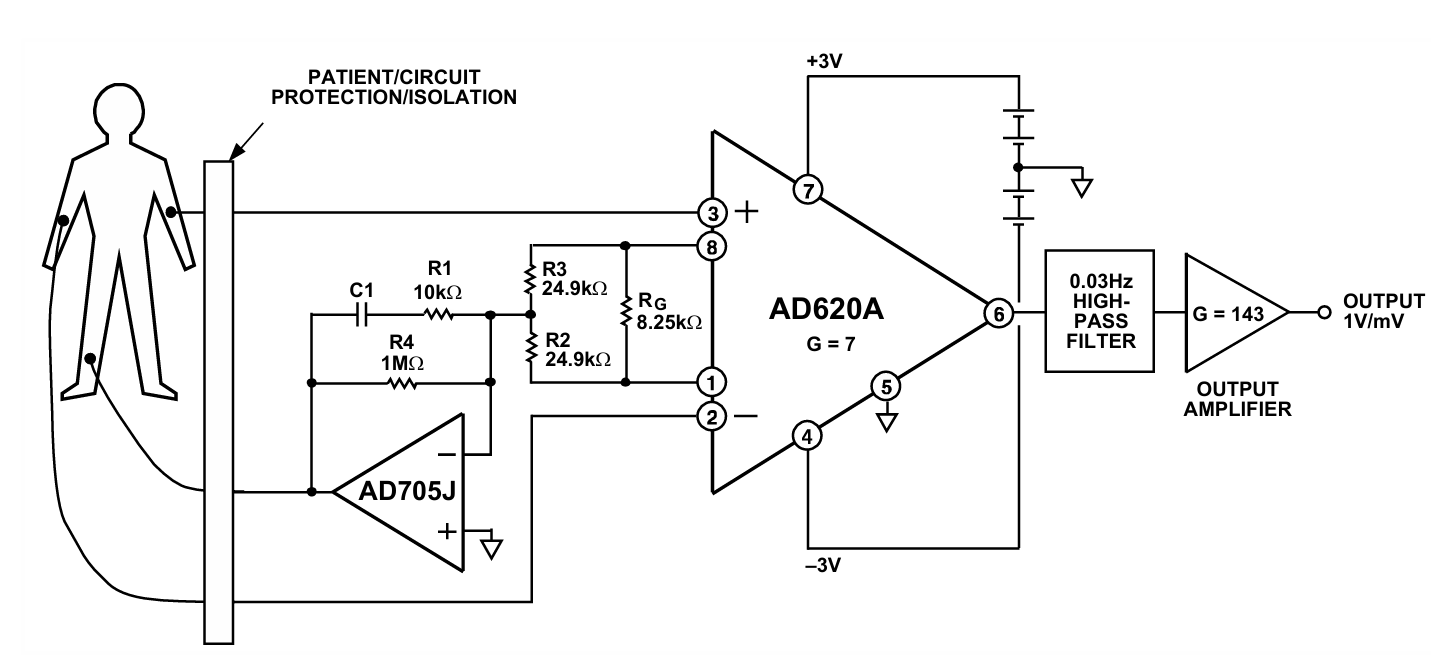
\includegraphics[width=0.6\textwidth]{image21.png}
    \caption{AD620A在ECG测量中的典型应用原理图}
    \label{F.ECG_image21}
\end{figure}


噪声抑制环节采用复合滤波策略,首先通过LM258DR中的单个运放构建了一个4元件SK型二阶低通滤波器,用于滤除108Hz以上的高频噪声,消除肌电等高频噪声干扰。如图\ref{F.ECG_image22}所示为SK型二阶低通滤波器的原理图,通过配置R50=10kΩ,R51=10kΩ,C75=220nF,C77=100nF,如式子\ref{E.108Hzfliter}所示,计算得知实现了约等于108Hz的特征频率,满足滤波需求。

\begin{equation}
    f_{0}=\frac{1}{2 \pi \sqrt{C_{75} C_{77} R_{50} R_{51}}}
\label{E.108Hzfliter}
\end{equation}

\begin{figure}[hbt]
    \centering
    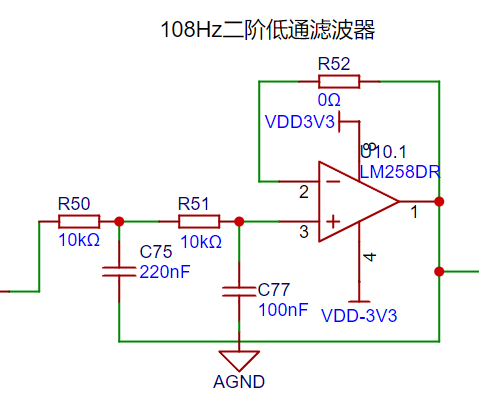
\includegraphics[width=0.6\textwidth]{image22.png}
    \caption{SK型二阶低通滤波器原理图}
    \label{F.ECG_image22}
\end{figure}

如图\ref{F.ECG_image24} \cite{新概念模拟电路3}为双T陷波器电路的示意图,通过使用LM258DR中的另一个运放构建了单运放双T网络有源陷波器,用于消除市电50Hz工频干扰,如图\ref{F.ECG_image23}所示为有源陷波器的原理图。通过如式子\ref{E.108Hzfliter}的计算可得,当R=6.8kΩ,C=470nF时,实现了约等于50Hz的特征频率,满足陷波需求。通过串联低通滤波器和陷波器,有效抑制了高频和工频噪声,保证了心电信号的准确采集。

\begin{figure}[hbt]
    \centering
    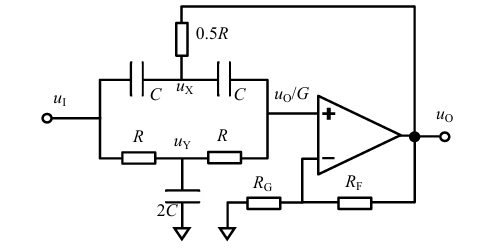
\includegraphics[width=0.6\textwidth]{image24.png}
    \caption{双T陷波器电路示意图}
    \label{F.ECG_image24}
\end{figure}

\begin{figure}[hbt]
    \centering
    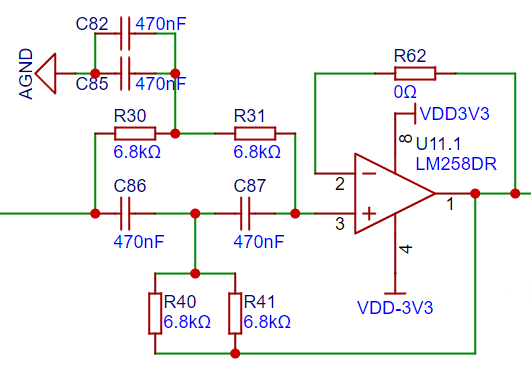
\includegraphics[width=0.6\textwidth]{image23.png}
    \caption{双T陷波器原理图}
    \label{F.ECG_image23}
\end{figure}

基线漂移问题通过RC高通网络(截止频率0.1Hz)解决,选用22μF陶瓷电容与51KΩ电阻构成一阶网络,在保证超低频衰减特性的同时避免极化效应。

信号调理链路末级采用两级反相放大器结构实现信号放大增益,先是通过一级反相放大电路,通过设置电阻Rf=100kΩ,Rin=2kΩ,使得一级放大电路反相放大信号50倍。再将放大后的信号经过50Hz双T陷波电路,滤除前级电路中微弱的工频干扰信号。最后通过反相加法器将信号放大5倍后叠加-1.65V偏置电压,使双极性心电信号适配3.3V单电源ADC的输入范围。输出级配置缓冲放大器隔离前后级阻抗,最终经AIN接口输出峰峰值达2.5V的调理信号。整个电路布局采用单点接地和屏蔽走线技术,关键模拟区域与数字电源域通过磁珠隔离,确保系统在复杂电磁环境下的稳定工作。如图\ref{F.ECG_image25}为心电信号采集与放大部分硬件原理图设计。

\begin{sidewaysfigure}
    \centering
    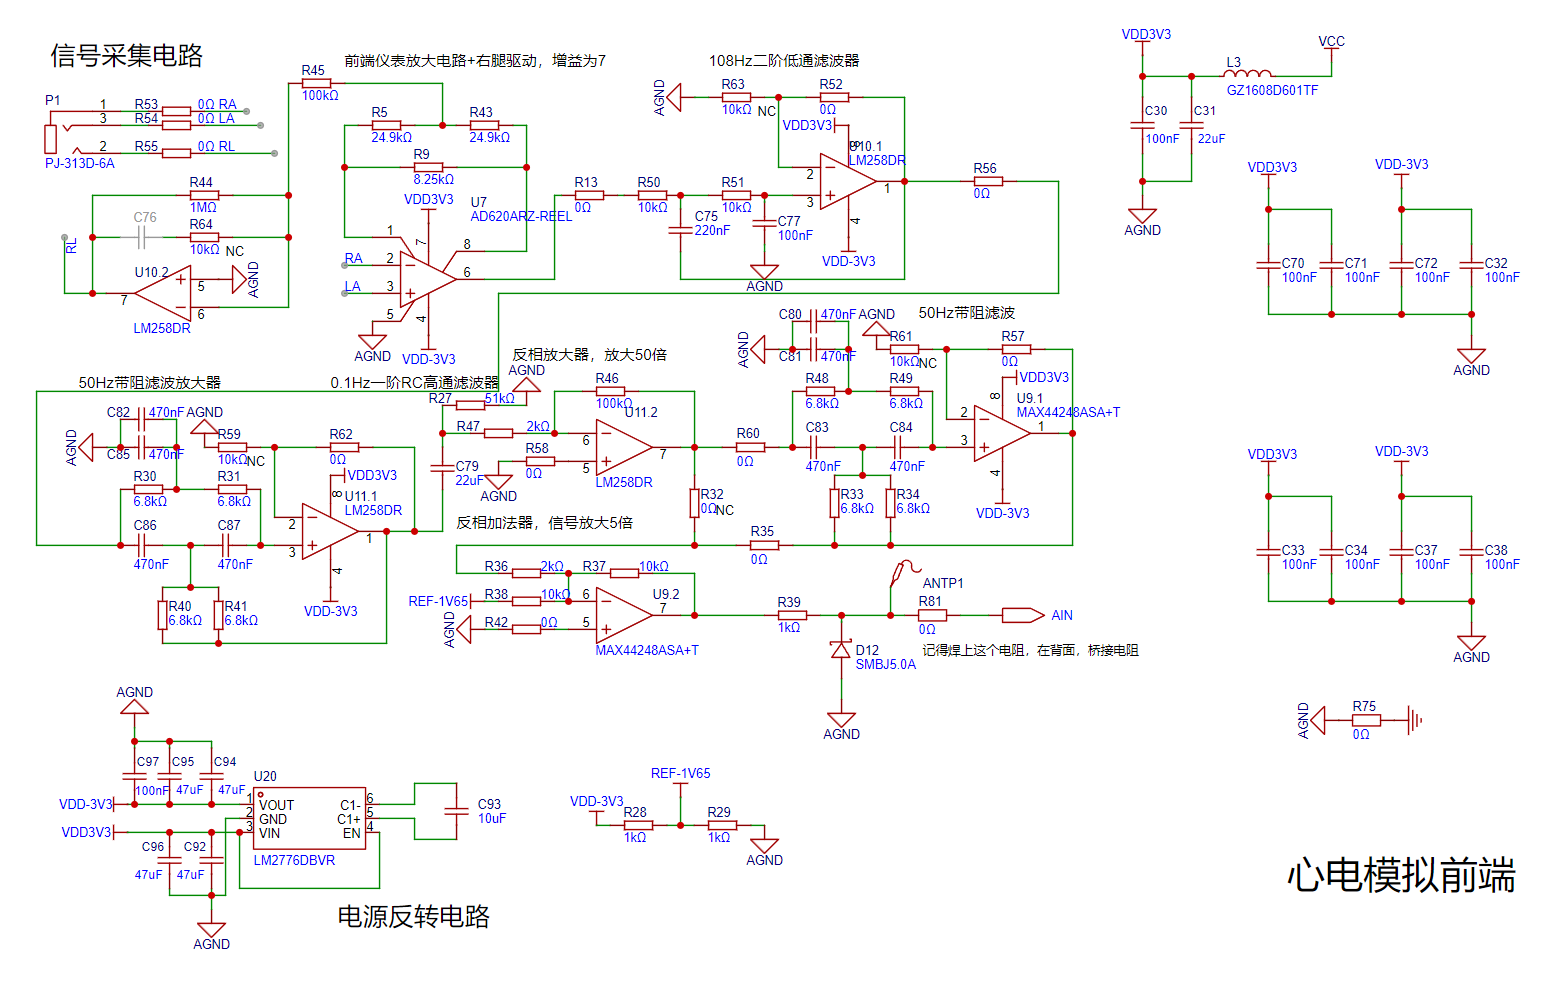
\includegraphics[width=1\textwidth]{image25.png}
    \caption{心电信号采集与放大部分硬件原理图设计}
    \label{F.ECG_image25}
\end{sidewaysfigure}

\newpage

\subsection{心电信号采集节点PCB设计}

在心电信号采集节点的PCB设计中,采用了两层板的结构,使用FR-4基材。重点研究了模拟电路与数字电路的布局和电源管理,以确保信号的完整性和系统的稳定性。

在布局设计中,心电采集的模拟电路部分与主控的数字电路部分被明确分区,分别放置在PCB的不同区域。有助于减少数字电路对模拟信号的干扰,特别是高频开关噪声对微弱心电信号的影响。为了模拟部分单点接地,两个区域的铺铜走地通过0Ω电阻连接,形成单点接地,有效地避免了地环路的产生,减少了地电位差异带来的干扰。防止了数字电路中的高频开关噪声通过地平面耦合至模拟电路。

为了进一步降低数字电路对模拟电路的干扰,特别是在主控MCU发射无线射频信号时,在电源供电上通过磁珠对两者进行隔离。磁珠在高频下表现出一定的高阻抗特性,能够有效抑制高频噪声的传导。

如图\ref{F.ECG_image26} \ref{F.ECG_image27}为心电信号采集节点PCB设计图。

\begin{figure}[hbt]
    \centering
    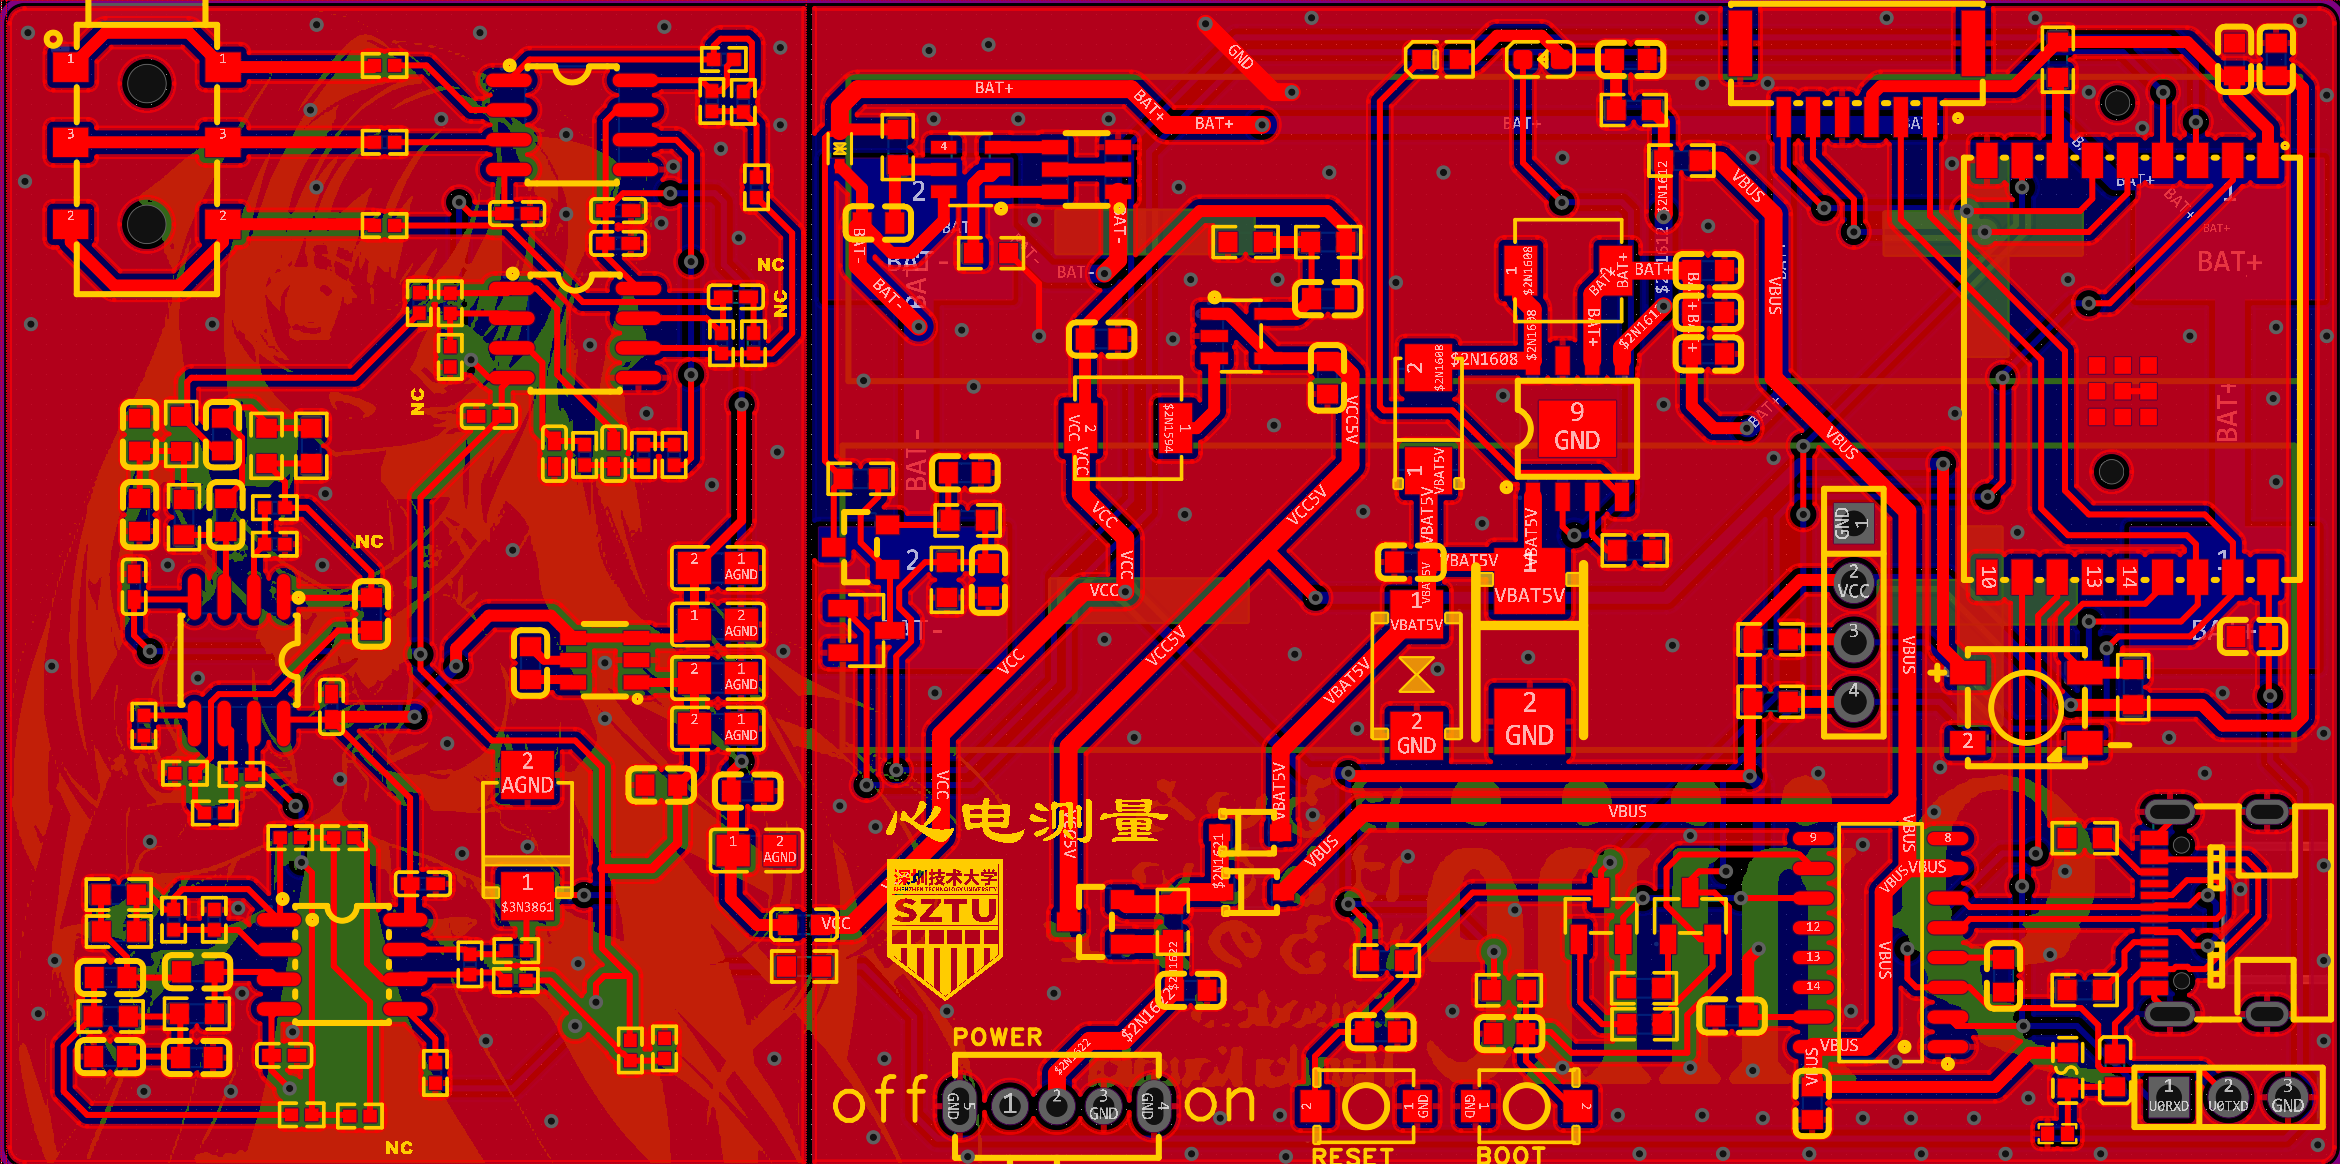
\includegraphics[width=0.8\textwidth]{image26.png}
    \caption{心电信号采集节点PCB顶层设计图}
    \label{F.ECG_image26}
\end{figure}

\begin{figure}[hbt]
    \centering
    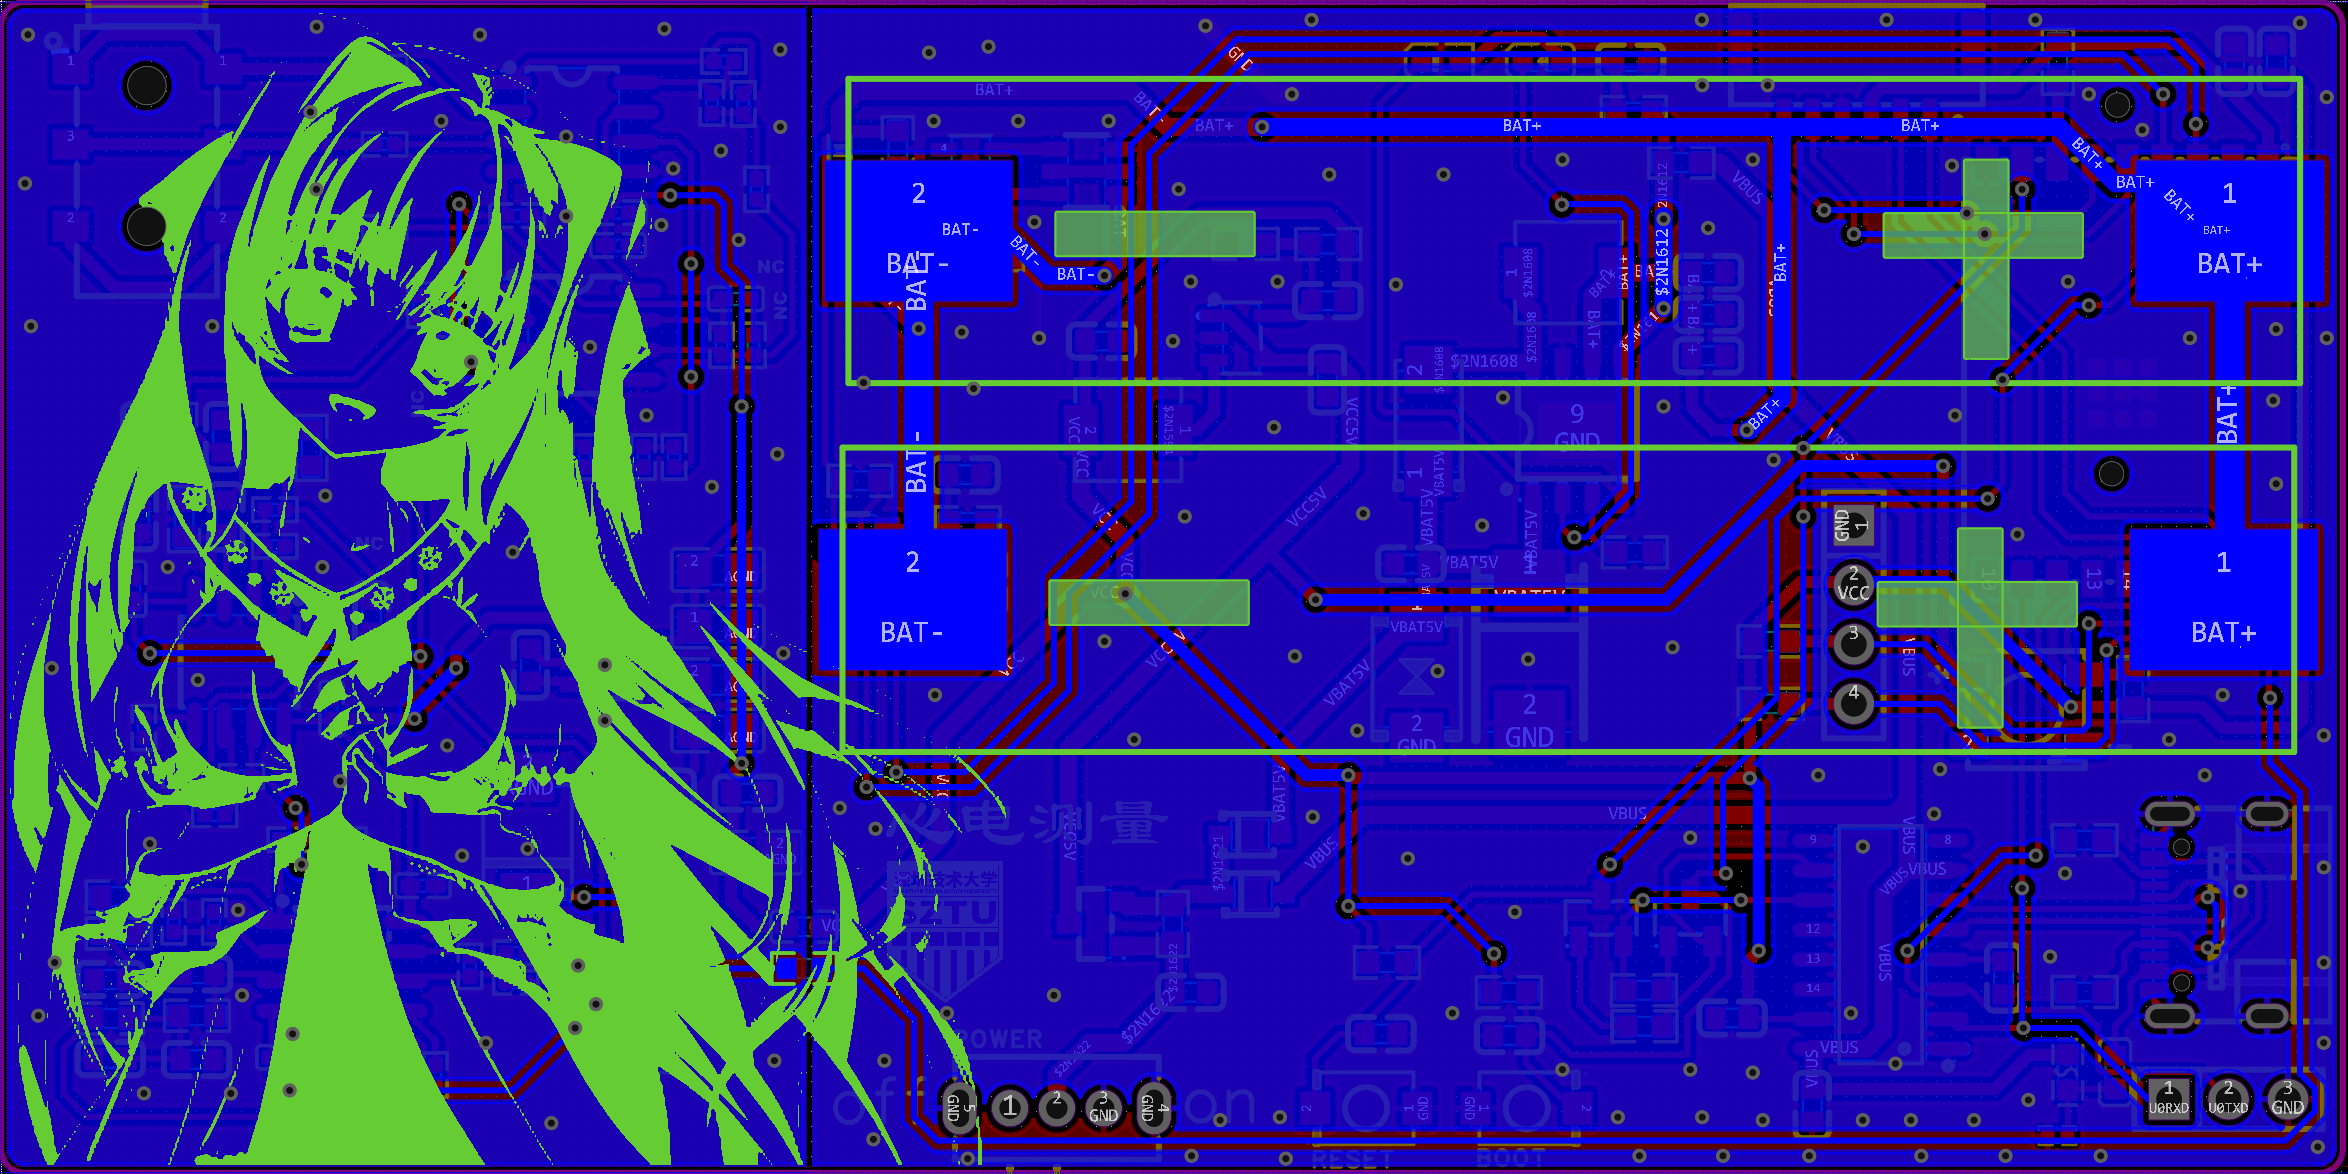
\includegraphics[width=0.8\textwidth]{image27.png}
    \caption{心电信号采集节点PCB底层设计图}
    \label{F.ECG_image27}
\end{figure}

为提高芯片散热效果和提升良好接地,TP5400与主控ESP32C3模组均以直连方式连接顶层铺铜GND。如图\ref{F.ECG_image28}所示。

\begin{figure}[!htb]
    \centering
    \begin{subfigure}[t]{0.24\linewidth}
        \begin{minipage}[b]{1\linewidth}
        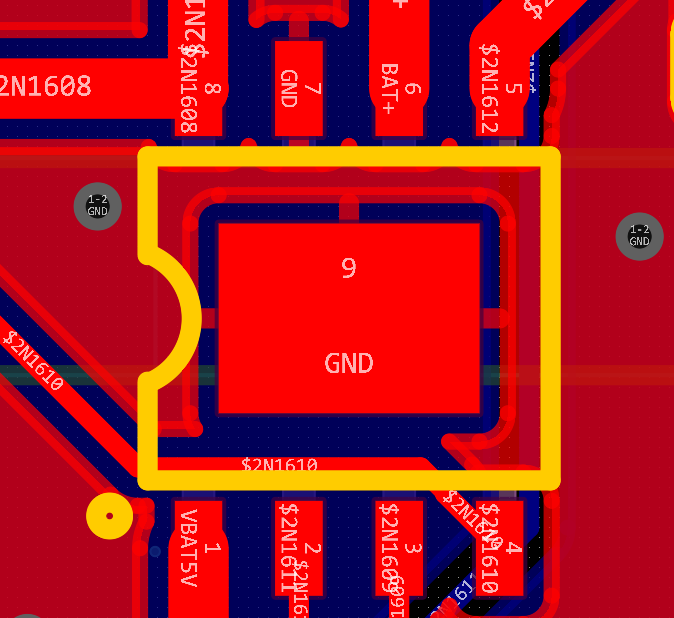
\includegraphics[width=1\linewidth]{image28.png}
        \caption{发散铺铜连接}
        \end{minipage}
    \end{subfigure}
    \begin{subfigure}[t]{0.24\linewidth}
        \begin{minipage}[b]{1\linewidth}
        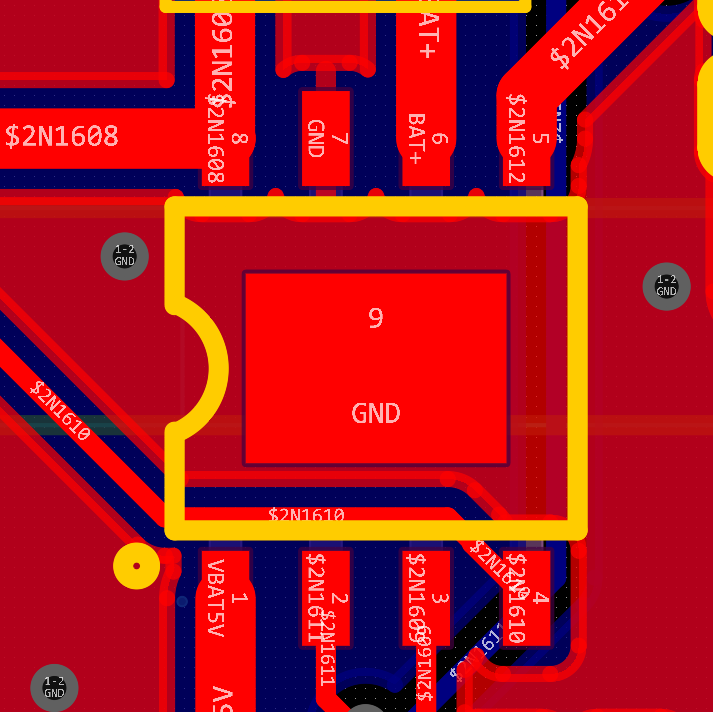
\includegraphics[width=1\linewidth]{image29.png}
        \caption{直连铺铜连接}
        \end{minipage}
    \end{subfigure}
    \caption{铺铜连接方式示意图}
    \label{F.ECG_image28}
\end{figure}

如图\ref{F.ECG_image30} MIFA天线是一种常用于小型化设备的天线类型,其结构紧凑,适用于空间受限的应用场景。然而,板载MIFA天线可能会受到设备外壳和PCB设计的影响,导致无线射频信号的性能下降。

因此在主控模块的选型过程中,选择了不带板载MIFA(蛇形倒F)天线而是仅带有IPEX-1接口的型号。

为提升信号接收效率,设计中通过模块引出的IPEX-1接口(如图\ref{F.ECG_image31} 为IPEX-1接口尺寸图)连接2.4GHz的FPC增益天线。IPEX接口是一种微型射频连接器,具有体积小、连接可靠的特点,广泛应用于需要高频信号传输的设备中。

FPC天线则具有良好的力学以及射频性能,能够适应多种安装环境,同时提供较高的增益,提升信号的接收和发射性能。将天线外置的设计策略,有助于减少设备外壳和PCB布局对无线射频信号的屏蔽和干扰。外置天线可以远离主板上的噪声源,降低电磁干扰的影响,从而提高通信的稳定性和可靠性。

\begin{figure}[htb]
    \centering
    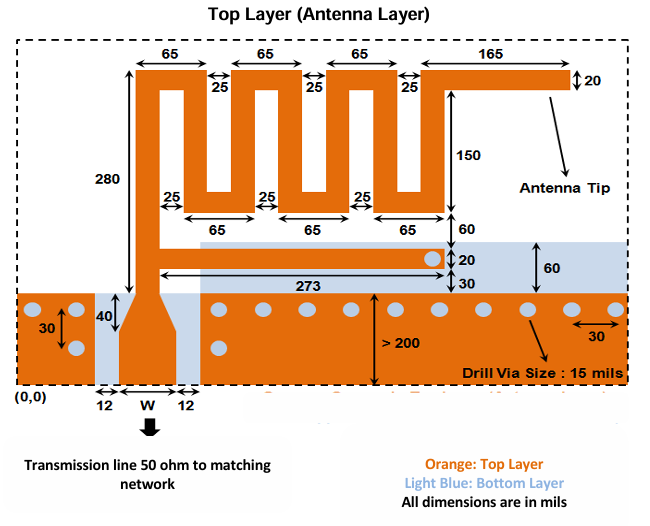
\includegraphics[width=0.6\textwidth]{image30.png}
    \caption{MIFA天线示意图}
    \label{F.ECG_image30}
\end{figure}

\begin{figure}[htb]
    \centering
    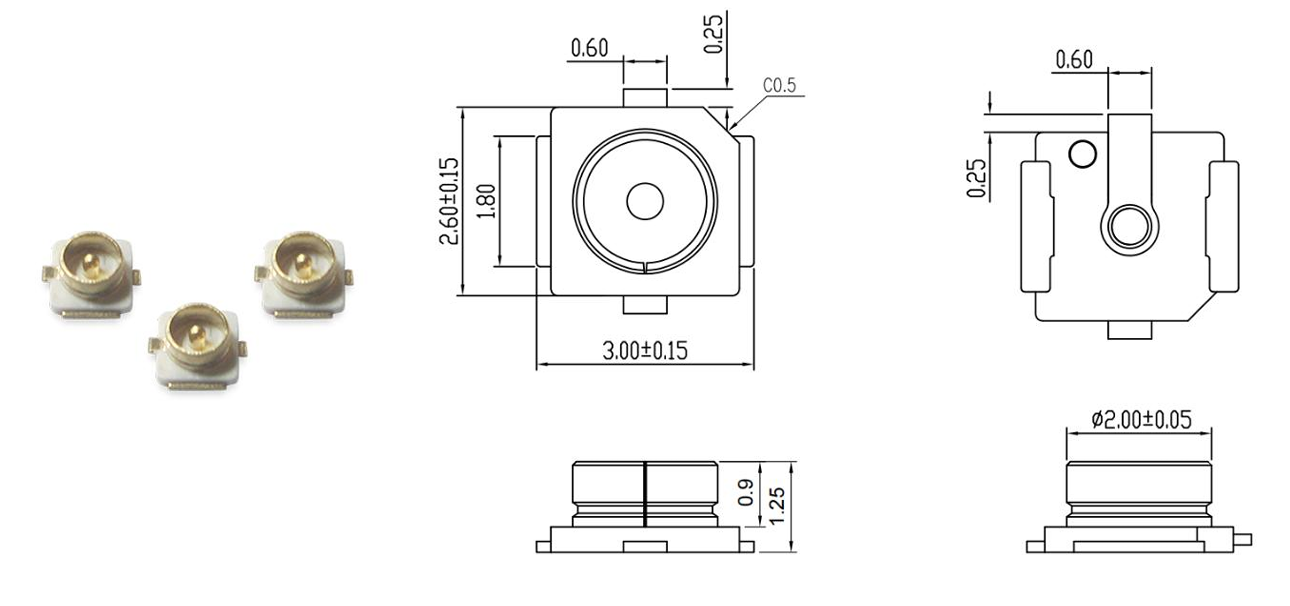
\includegraphics[width=0.6\textwidth]{image31.png}
    \caption{IPEX-1接口尺寸图\cite{IPEX-1}}
    \label{F.ECG_image31}
\end{figure}

\begin{figure}[H]
    \centering
    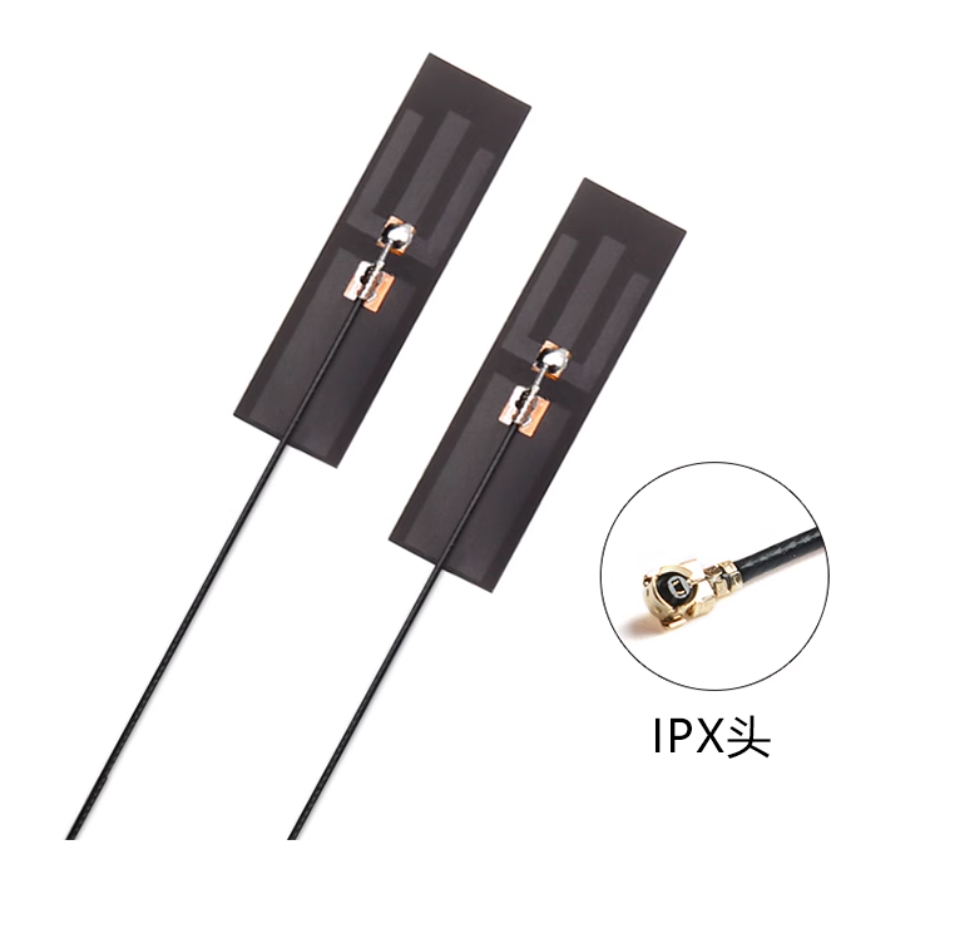
\includegraphics[width=0.4\textwidth]{image32.png}
    \caption{FPC天线实物图}
    \label{F.ECG_image32}
\end{figure}

如图\ref{F.ECG_image33}为节点设备通过嘉立创打样并完成元件焊接与调试的PCBA实物图。

\begin{figure}[htb]
    \centering
    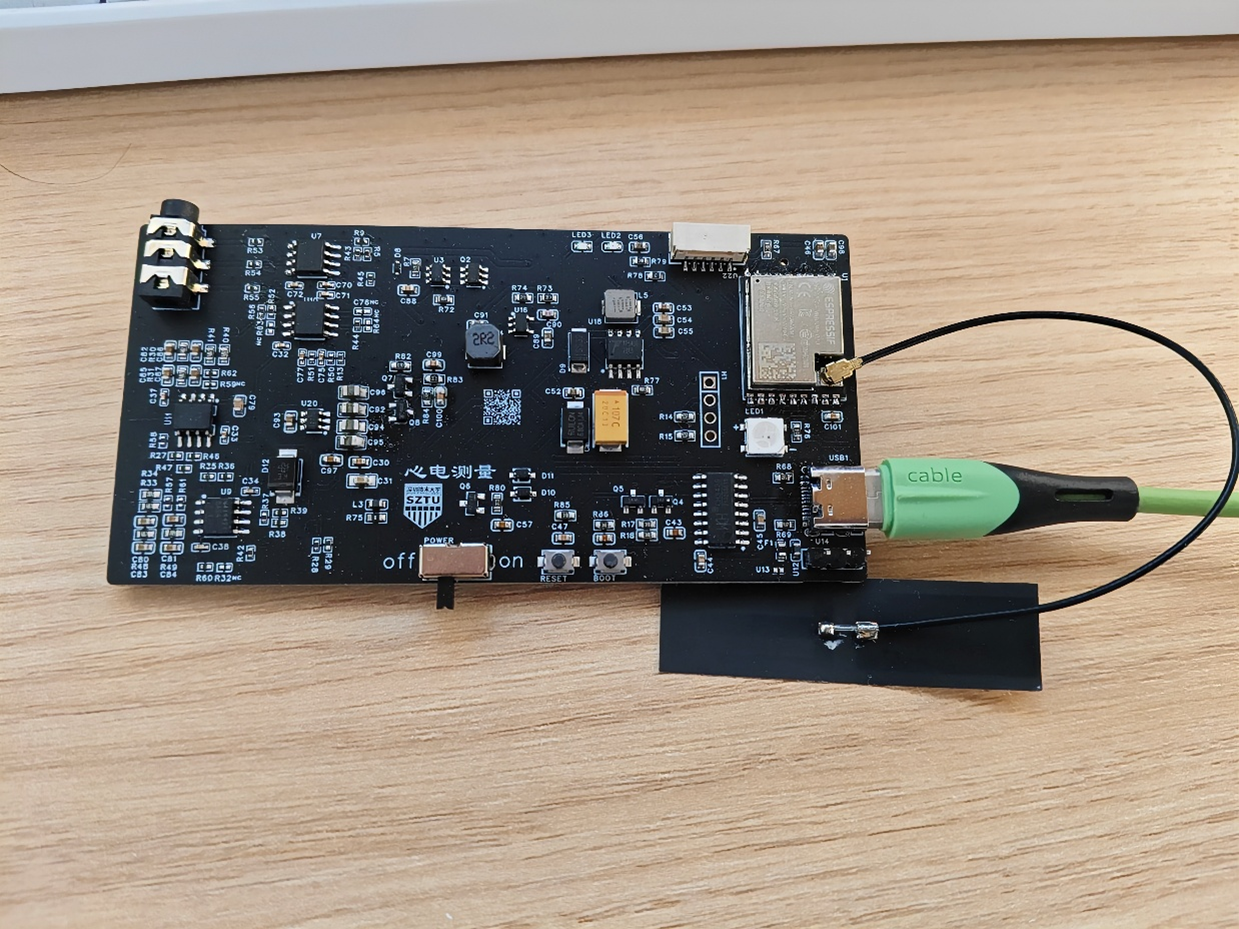
\includegraphics[width=1\textwidth]{image33.png}
    \caption{心电采集节点PCBA实物图}
    \label{F.ECG_image33}
\end{figure}

\subsection{心电信号采集基站硬件设计}

由于节点设备开发时间耗时较长,出于在硬件设计部分的时间成本考虑,本研究在心电采集设备的基站端选择使用嘉立创公司出品的立创·实战派ESP32-C3开发板作为心电采集设备的基站开发平台。

该开发板相较于那些用于学习的开发板,更趋近于实际产品的外观,体积小巧,仅有69×41×12mm大小,不仅内部集成了姿态传感器、地磁传感器、温湿度传感器等,还具备2英寸LCD彩屏以及贴片麦克风作为音频输入和一个2W的喇叭作为音频输出。开发板集成了Wi-Fi和蓝牙功能,并预留了两个拓展接口,便于连接更多外部传感器模块和执行器。

此开发板的光固化打印的壳体采用了无螺丝的设计,便于快速拆装,有助于加速开发进程。综合考虑其丰富的功能集成、紧凑的设计以及易于使用的特性,立创·实战派ESP32-C3开发板成为了笔者在有限时间内实现心电采集基站端开发的理想选择。 如图\ref{F.ECG_image34}为立创·实战派ESP32-C3开发板PCBA图。

\begin{figure}[htb]
    \centering
    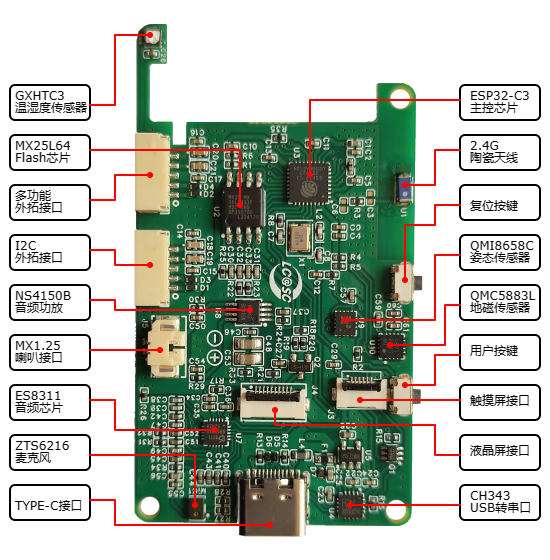
\includegraphics[width=0.6\textwidth]{image34.png}
    \caption{立创·实战派ESP32-C3开发板PCBA图}
    \label{F.ECG_image34}
\end{figure}

\section{软件部分设计与实现}

如图\ref{F.ECG_image37}为心电同步采集设备运行流程泳道图。心电同步采集设备的软件设计主要包括心电信号采集节点软件设计、心电信号采集基站软件设计和心电信号采集设备上位机软件设计三个部分。

\begin{sidewaysfigure}
    \centering
    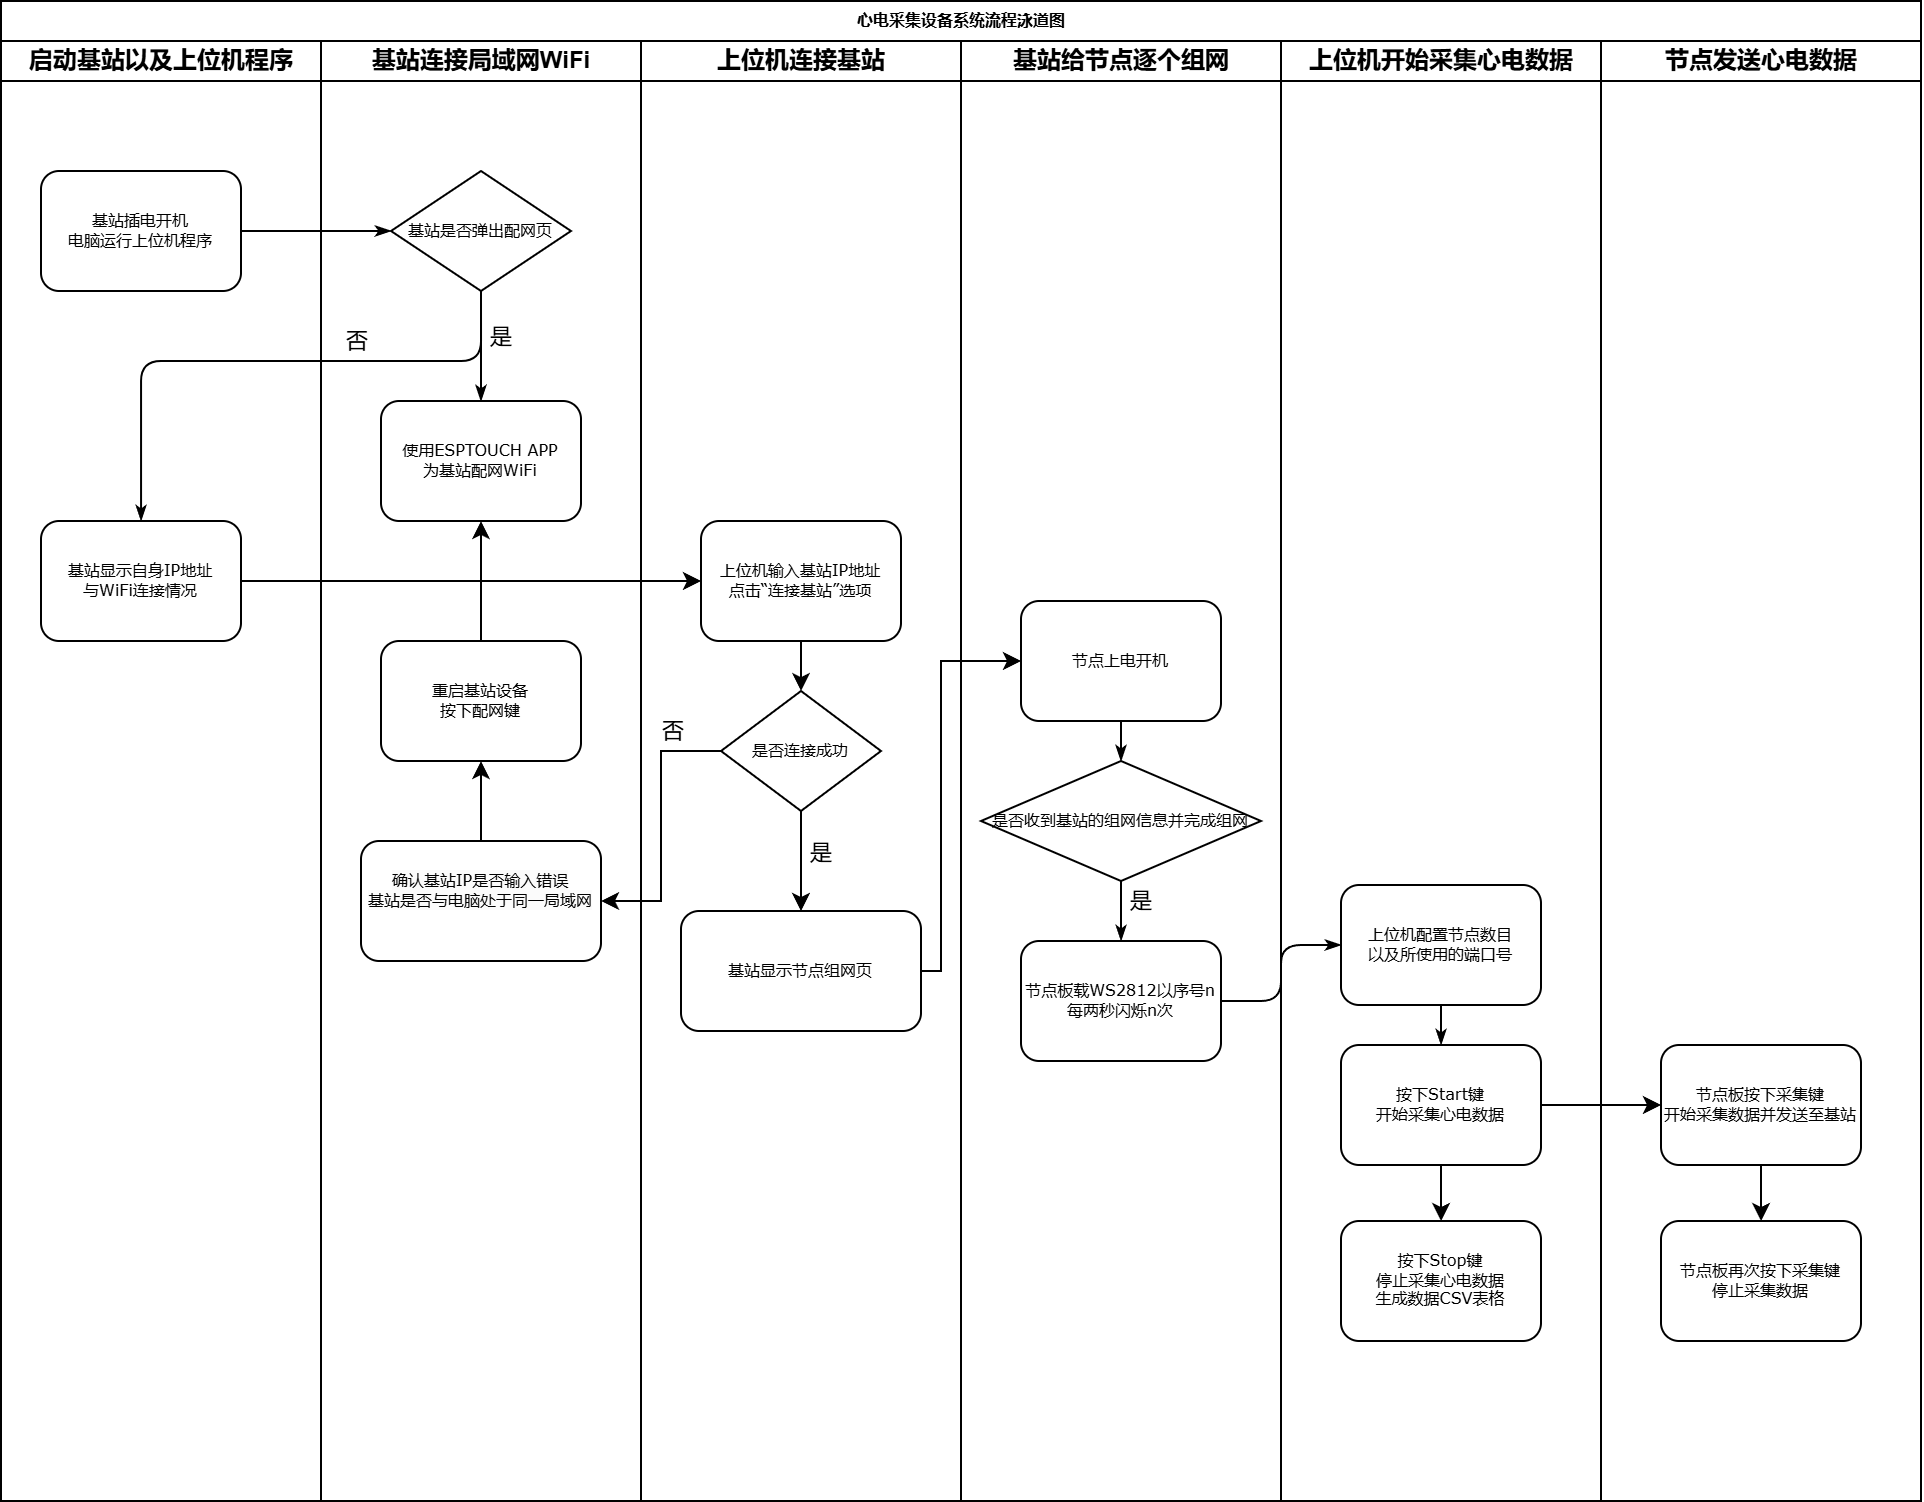
\includegraphics[width=0.8\textwidth]{image37.png}
    \caption{心电同步采集设备运行流程泳道图}
    \label{F.ECG_image37}
\end{sidewaysfigure}

\subsection{心电信号采集节点软件设计}

在心电采集节点的软件设计中,采用了乐鑫科技(Espressif)提供的物联网开发框架 ESP-IDF(Espressif IoT Development Framework)作为软件开发SDK(Software Develop Kit),选用了稳定版本 V5.3.0。ESP-IDF 是一个开源的实时操作系统开发框架,专为 ESP32 系列芯片设计,提供了丰富的库和组件,支持 Wi-Fi、蓝牙、以太网等多种连接方式,以及各种外设驱动和协议栈。该框架采用 CMake 作为构建系统,确保了项目的模块化、跨平台开发并提高了软件可维护性。如图\ref{F.ECG_image35}为ESP-IDF工作流程图。

\begin{figure}[H]
    \centering
    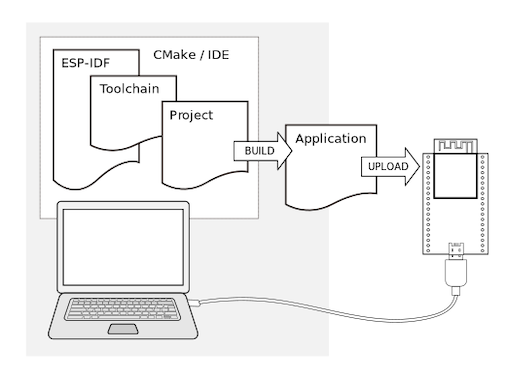
\includegraphics[width=0.6\textwidth]{image35.png}
    \caption{ESP-IDF工作流程图\cite{espressif2025espidf}}
    \label{F.ECG_image35}
\end{figure}

在软件架构方面,ESP-IDF基于 FreeRTOS 实时操作系统实现多任务管理的效果。FreeRTOS 是一个小巧且高效的实时内核,支持多任务调度、任务间通信、同步机制等。FreeRTOS 采用抢占式的调度策略,辅以时间片轮转机制。每个任务在创建时被人为地分配一个固定的优先级,调度器根据这些优先级和任务状态(如就绪、运行、阻塞、挂起)来决定各任务的执行顺序。当高优先级任务进入就绪状态时,调度器会立即抢占当前正在运行的低优先级任务,确保高优先级任务得到及时执行。

由于ESP32-C3为单核RISC-V处理器,在单核 MCU 上运行多个任务时,任务的上下文切换和其他任务的执行会占用一定的 CPU 时间,会对ADC 测量这种高频任务的实际运行频率产生影响。为此,通过对各任务的优先级和执行时间进行了精细的调度和优化,确保在执行如 UDP 发送、WS2812 控制这种低频任务时,对高频任务的影响降至最低。通过对采集的心电数据进行分析,验证了实际的 ADC 测量频率达到 991 Hz,充分满足心电数据采集的需求。测试数据如图\ref{F.ECG_image38}所示。

\begin{figure}[htb]
    \centering
    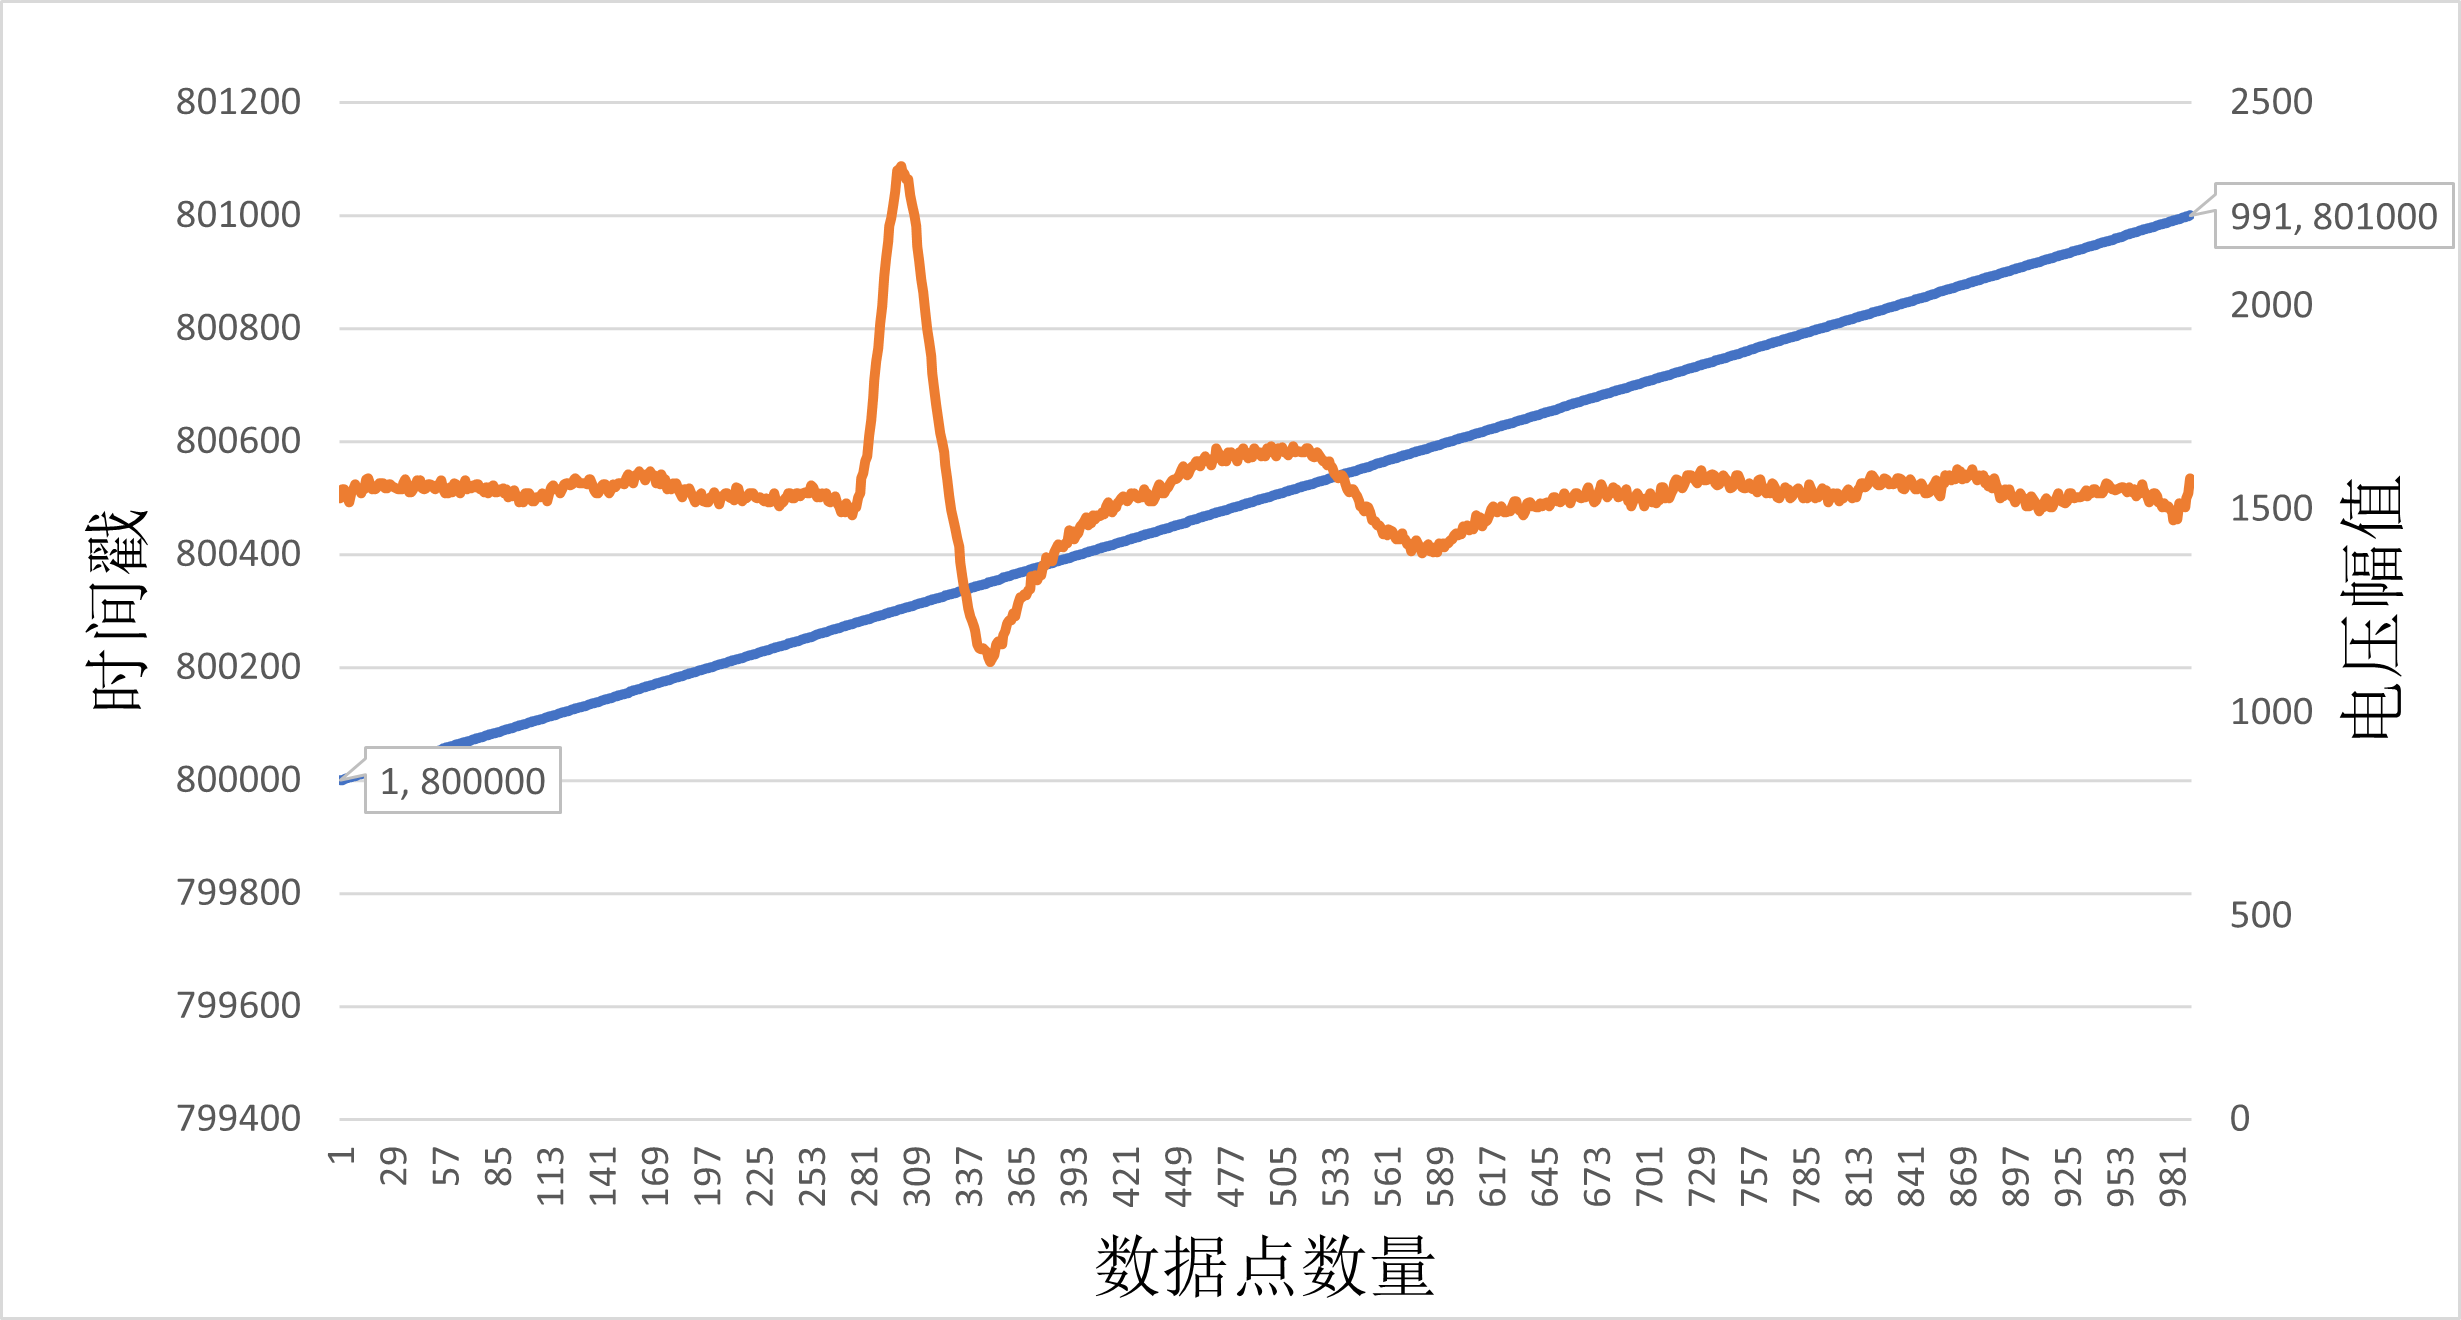
\includegraphics[width=0.8\textwidth]{image38.png}
    \caption{1s内所采心电数据频率统计图}
    \label{F.ECG_image38}
\end{figure}

在具体实现上,采集节点的软件包含以下主要功能模块:

\begin{enumerate}
    \item \textbf{WiFi 基带控制任务}:负责管理 WiFi 的底层操作,包括连接建立、数据传输等,确保设备能够稳定地进行无线通信。同时包括控制ESP-NOW协议的初始化和数据传输、控制WiFi基带连接局域网无线路由器WiFi的功能、DHCP获取IP地址以及网络掉线重连等功能。
    
    \item \textbf{ESPNOW 组网任务}:利用乐鑫定义的基于数据链路层的无线通信协议 ESP-NOW,实现设备间的高效通信。该协议无需路由器即可实现单对多、多对多的设备连接和控制,通过ESP-NOW向基站注册本机设备并获取局域网WiFi信息以及时间同步偏移量,当完成组网后该任务销毁以节省资源占用。

    \item \textbf{ADC 测量任务}:该任务以理论上的 1000 Hz 频率运行,负责调用ADC实时采集心电信号并将所采集的心电信号ADC值计算成实际电压幅值,再为数据打上测量时的实时时间戳,通过FreeRTOS的消息队列功能将每次测量的数据包发至心电数据消息队列中。通过优化代码和合理分配系统资源,实际测量频率达到约 992 Hz,满足心电监测的精度要求。
    
    \item \textbf{UDP 数据发送任务}:从心电数据消息队列中取出数据,将队列中各数据序列化,形成数据帧,通过 UDP 协议将数据帧发送到上位机程序,实现数据的实时传输。

    \item \textbf{WS2812 驱动任务}:控制 WS2812 LED 灯的显示,以提供视觉反馈或状态指示。在等待组网时红灯常亮,组网并连接WiFi成功后每2s按节点序号控制WS2812按节点序规律闪烁绿灯,当节点设备低电池电量时红灯呼吸闪烁
\end{enumerate}

如图\ref{F.ECG_image36}为心电信号采集节点软件架构图。

\begin{figure}[htb]
    \centering
    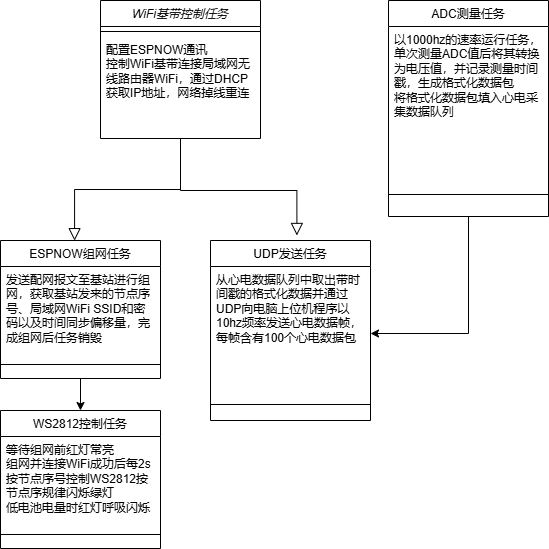
\includegraphics[width=0.8\textwidth]{image36.png}
    \caption{心电信号采集节点软件架构图}
    \label{F.ECG_image36}
\end{figure}

在无线多设备心电图(ECG)采集系统中,确保各节点设备所采心电数据的时序同步对于实现实时重放和准确分析至关重要。由于节点间无法做到同时上电,节点设备间的内置时钟会有巨大差异,将造成各节点所采集的 ECG 数据时间戳不一致的问题。为解决这一问题,本研究设计了一种基于时间戳同步和统一时钟同步的策略。在该策略中,各节点通过基站设备建立无线采集网络,由基站设备在配网时当节点加入到采集网络中时对其进行授时,建立基于基站设备时序的统一时间基准,确保各设备异步采集的数据在时间戳上具有一致性。

具体而言,节点设备在等待配网的阶段,通过ESP-NOW向基站发起配网请求。基站设备接收到节点设备的配网请求后,在为该节点分配节点序号的同时,将基站此时的时间戳添加到配网数据包中,向发起配网申请的节点单播发送配网数据包。节点设备在收到给自己的配网数据包后,通过设置时钟偏移量来校准自身时钟,以确保与基站设备保持一致。在数据采集过程中,各节点设备为每条 ECG 数据添加基于校准时钟的时间戳。在数据汇总阶段,上位机只需要根据时间戳对来自不同设备的数据进行排序和融合,确保多设备采集的数据在时间轴上准确对齐,实现同步重放和分析。通过上述时间同步策略的设计与实现,确保了无线多设备 ECG 采集系统中各设备数据的时序一致性,提高了数据的准确性和可靠性,为后续的实时重放和分析提供了坚实的基础。 


\newpage    % 两个章节之间分页,不想分的话可注释掉


\section{总结与展望}

\noindent{纯数字编号}
\begin{enumerate}
 \item XXXXXXXXXX
 \label{item1}
 \item XXXXXXXXXX
 \item XXXXXXXXXX
\end{enumerate}
罗马编号
\begin{enumerate}[label=(\roman*)]
 \item XXXXXXXXXX
 \label{item2}
 \item XXXXXXXXXX
 \item XXXXXXXXXX
\end{enumerate}
括号编号
\begin{enumerate}[label=(\arabic*)]
 \item XXXXXXXXXX
 \label{item3}
 \item XXXXXXXXXX
 \item XXXXXXXXXX
\end{enumerate}
半括号编号
\begin{enumerate}[label=\arabic*)]
 \item XXXXXXXXXX
 \label{item4}
 \item XXXXXXXXXX
 \item XXXXXXXXXX
\end{enumerate}
小字母编号
\begin{enumerate}[label=\alph*)]
 \item XXXXXXXXXX
 \label{item5}
 \item XXXXXXXXXX
 \item XXXXXXXXXX
\end{enumerate}

引用测试,正如~\ref{item1}、\ref{item2}、\ref{item3}、\ref{item4}、\ref{item5} 所示

\subsection{工作展望}
手动编号 %(不推荐,无法被交叉引用)

本课题针对XX,鉴于XXX,对XX进行了提高,但是XXX,所以有如下XX:

(1)目前XX虽然XX,但是XX仍然XX,所以XX仍然是一个值得XX的问题。

(2)随着XX,XX具有XX的问题,仍值得进一步XX。

(3)本课题在XX有了XX,但是XX的XX还存在XX,所以XX。


\newpage
